\documentclass[12pt]{article} % use larger type; default would be 10pt

\usepackage{tikz}
\usepackage{pgfplots}
\usetikzlibrary{calc}
\usetikzlibrary{arrows}
\usetikzlibrary{patterns}
        \newcommand\degree[0]{^{\circ}}
\usetikzlibrary{shapes.misc}

\title{Play with TikZ}
\author{Just Us}
%\date{} % Activate to display a given date or no date (if empty),
         % otherwise the current date is printed 

\begin{document}
\maketitle

\section{Chap 6 Radians}



ch6-4

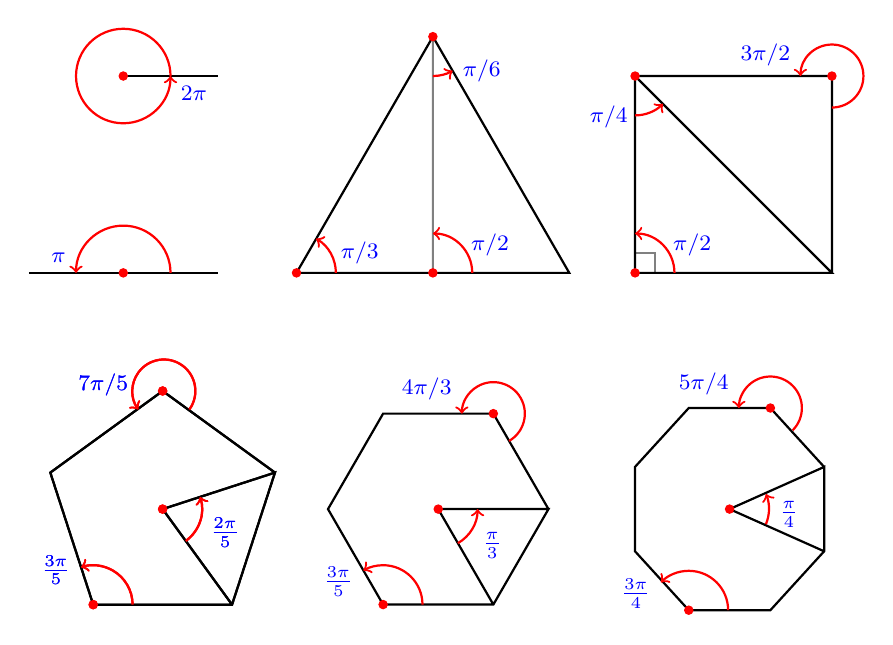
\begin{tikzpicture} 
\coordinate (O) at (0,0);
\coordinate (A) at (0,2.5);
\draw[black, thick] (A)--++(1.2,0);
\filldraw[red] (A) circle (1.5pt);
\draw[red, thick, ->] (.6,2.5) arc (0:360:.6cm) node[below right]{\color{blue}\footnotesize $2\pi$};

%second fig
\draw[black, thick] (-1.2,0)--(1.2,0);
\filldraw[red] (O) circle (1.5pt);
\draw[red, thick, ->] (.6,0) arc (0:180:.6cm) node[above left]{\color{blue}\footnotesize $\pi$};

%third fig
\coordinate (O) at (2.2,0);
\coordinate (A) at ($ (O) + 2*sqrt(3)*(1,0) $);
\coordinate (B) at ($ (A)+ sqrt(3)*(-1,0)+(0,3) $);
\coordinate (C) at ($ (O)+ sqrt(3)*(1,0) $);
\draw[black, thick] (O)--(A) -- (B)--(O);
\draw[gray, thick] (B)--(C);
\filldraw[red] (O) circle (1.5pt);
\draw[red, thick, ->] (2.7,0) arc (0:60:.5cm) node[right, midway]{\color{blue}\footnotesize $\pi/3$};
\filldraw[red] (C) circle (1.5pt);
\draw[red, thick, ->] ($ (C) + (.5,0) $) arc (0:90:.5cm) node[right, midway]{\color{blue}\footnotesize $\pi/2$};
\filldraw[red] (B) circle (1.5pt);
\draw[red, thick, ->] ($ (B) + (0, -.5) $) arc (-90:-60:.5cm) node[ right, ]{\color{blue}\footnotesize $\pi/6$};

%fourth fig
\coordinate (O) at (6.5,0);
\coordinate (A) at ($ (O) +(2.5,0) $);
\coordinate (B) at ($ (A)+ (0,2.5) $);
\coordinate (C) at ($ (O) + (0,2.5) $);
\draw[gray, thick] (O) rectangle ++(.25,.25);
\draw[black, thick] (A) -- (B)-- (C)--(O)--(A)--(C);

\filldraw[red] (O) circle (1.5pt);
\draw[red, thick, ->] ($ (O) + (.5,0)$) arc (0:90:.5cm) node[right, midway]{\color{blue}\footnotesize $\pi/2$};
\filldraw[red] (C) circle (1.5pt);
\draw[red, thick, ->] ($ (C) + (0,-.5)$) arc (-90:-45:.5cm) node[anchor=north east, xshift=-9, yshift=3]{\color{blue}\footnotesize $\pi/4$};
\filldraw[red] (B) circle (1.5pt);
\draw[red, thick, ->] ($ (B) + (0,-.4)$) arc (-90:180:.4cm) node[anchor=south east, ]{\color{blue}\footnotesize $3\pi/2$};

%fifth fig
\coordinate (O) at (.5,-3);
\coordinate (A) at ($ (O) +1.5*(0,1) $);
\coordinate (B) at ($ (O)+1.5*cos(72)*(0,1) +1.5*sin(72)*(-1,0) $);
\coordinate (C) at ($ (O)+1.5*cos(36)*(0,-1) +1.5*sin(36)*(-1,0) $);
\coordinate (D) at ($ (O)+1.5*cos(36)*(0,-1) +1.5*sin(36)*(1,0) $);
\coordinate (E) at ($ (O)+1.5*cos(72)*(0,1) +1.5*sin(72)*(1,0) $);

\draw[black, thick] (E)--(A)-- (B)-- (C)--(D)--(E)--(O)--(D);

\filldraw[red] (O) circle (1.5pt);
\draw[red, thick, ->] ($ (O) + .5*sin(36)*(1,0) + .5*cos(36)*(0,-1)$) arc (-54:18:.5cm) node[right, midway, yshift=-4]{\color{blue}\small $\frac{2\pi}{5}$};
\filldraw[red] (C) circle (1.5pt);
\draw[red, thick, ->] ($ (C) + (.5,0)$) arc (0:108:.5cm) node[anchor=north east, yshift=8]{\color{blue}\small $\frac{3\pi}{5}$};
\filldraw[red] (A) circle (1.5pt);
\draw[red, thick, ->] ($ (A) + 0.4*sin(36)*(0,-1) + .4*cos(32)*(1,0)$) arc (-36:216:.4cm) node[anchor=south east, yshift=1]{\color{blue}\footnotesize $7\pi/5$};

%sixth fig
\coordinate (O) at (4,-3);
\coordinate (A) at ($ (O) +1.4*(1,0) $);
\coordinate (B) at ($ (O)+1.4*cos(60)*(1,0) +1.4*sin(60)*(0,1) $);
\coordinate (C) at ($ (O)+1.4*cos(60)*(-1,0) +1.4*sin(60)*(0,1) $);
\coordinate (D) at ($ (O)+1.4*(-1,0) $);
\coordinate (E) at ($ (O)+1.4*cos(60)*(-1,0) +1.4*sin(60)*(0,-1) $);
\coordinate (F) at ($ (O)+1.4*cos(60)*(1,0) +1.4*sin(60)*(0,-1) $);

\draw[black, thick] (A)-- (B)-- (C)--(D)--(E)--(F)--(A)--(O)--(F);

\filldraw[red] (O) circle (1.5pt);
\draw[red, thick, <-] ($ (O) + .5*(1,0) $) arc (0:-60:.5cm) node[right, midway, yshift=-6]{\color{blue}\small $\frac{\pi}{3}$};
\filldraw[red] (E) circle (1.5pt);
\draw[red, thick, ->] ($ (E) + (.5,0)$) arc (0:120:.5cm) node[left, yshift=-4]{\color{blue}\small $\frac{3\pi}{5}$};
\filldraw[red] (B) circle (1.5pt);
\draw[red, thick, ->] ($ (B) + 0.4*sin(60)*(0,-1) + .4*cos(60)*(1,0)$) arc (-60:180:.4cm) node[anchor=south east, yshift=1]{\color{blue}\footnotesize $4\pi/3$};


%fifth fig
\coordinate (O) at (.5,-3);
\coordinate (A) at ($ (O) +1.5*(0,1) $);
\coordinate (B) at ($ (O)+1.5*cos(72)*(0,1) +1.5*sin(72)*(-1,0) $);
\coordinate (C) at ($ (O)+1.5*cos(36)*(0,-1) +1.5*sin(36)*(-1,0) $);
\coordinate (D) at ($ (O)+1.5*cos(36)*(0,-1) +1.5*sin(36)*(1,0) $);
\coordinate (E) at ($ (O)+1.5*cos(72)*(0,1) +1.5*sin(72)*(1,0) $);

\draw[black, thick] (E)--(A)-- (B)-- (C)--(D)--(E)--(O)--(D);

\filldraw[red] (O) circle (1.5pt);
\draw[red, thick, ->] ($ (O) + .5*sin(36)*(1,0) + .5*cos(36)*(0,-1)$) arc (-54:18:.5cm) node[right, midway, yshift=-4]{\color{blue}\small $\frac{2\pi}{5}$};
\filldraw[red] (C) circle (1.5pt);
\draw[red, thick, ->] ($ (C) + (.5,0)$) arc (0:108:.5cm) node[anchor=north east, yshift=8]{\color{blue}\small $\frac{3\pi}{5}$};
\filldraw[red] (A) circle (1.5pt);
\draw[red, thick, ->] ($ (A) + 0.4*sin(36)*(0,-1) + .4*cos(32)*(1,0)$) arc (-36:216:.4cm) node[anchor=south east, yshift=1]{\color{blue}\footnotesize $7\pi/5$};

%seventh fig
\coordinate (O) at (7.7,-3);
\coordinate (A) at ($ (O) +1.3*cos(22.5)*(1,0) +1.4*sin(22.5)*(0,1) $);
\coordinate (B) at ($ (O)+1.3*cos(66.5)*(1,0) +1.4*sin(66.5)*(0,1) $);
\coordinate (C) at ($ (O)+1.3*cos(66.5)*(-1,0) +1.4*sin(66.5)*(0,1) $);
\coordinate (D) at ($ (O) +1.3*cos(22.5)*(-1,0) +1.4*sin(22.5)*(0,1) $);
\coordinate (E) at ($ (O) +1.3*cos(22.5)*(-1,0) +1.4*sin(22.5)*(0,-1) $);
\coordinate (F) at ($ (O)+1.3*cos(66.5)*(-1,0) +1.4*sin(66.5)*(0,-1)  $);
\coordinate (G) at ($ (O)+1.3*cos(66.5)*(1,0) +1.4*sin(66.5)*(0,-1) $);
\coordinate (H) at ($ (O) +1.3*cos(22.5)*(1,0) +1.4*sin(22.5)*(0,-1) $);

\draw[black, thick] (A)-- (B)-- (C)--(D)--(E)--(F)--(G)--(H)--(A)--(O)--(H);

\filldraw[red] (O) circle (1.5pt);
\draw[red, thick, ->] ($ (O) + .5*cos(22.5)*(1,0)+ .5*sin(22.5)*(0,-1) $) arc (-22.5:22.5:.5cm) node[right, midway, yshift=-2]{\color{blue}\small $\frac{\pi}{4}$};
\filldraw[red] (F) circle (1.5pt);
\draw[red, thick, ->] ($ (F) + (.5,0)$) arc (0:135:.5cm) node[left, yshift=-4]{\color{blue}\small $\frac{3\pi}{4}$};
\filldraw[red] (B) circle (1.5pt);
\draw[red, thick, ->] ($ (B) + 0.4*sin(45)*(0,-1) + .4*cos(45)*(1,0)$) arc (-45:180:.4cm) node[anchor=south east, yshift=1]{\color{blue}\footnotesize $5\pi/4$};

\end{tikzpicture}
\newline

ch6-5

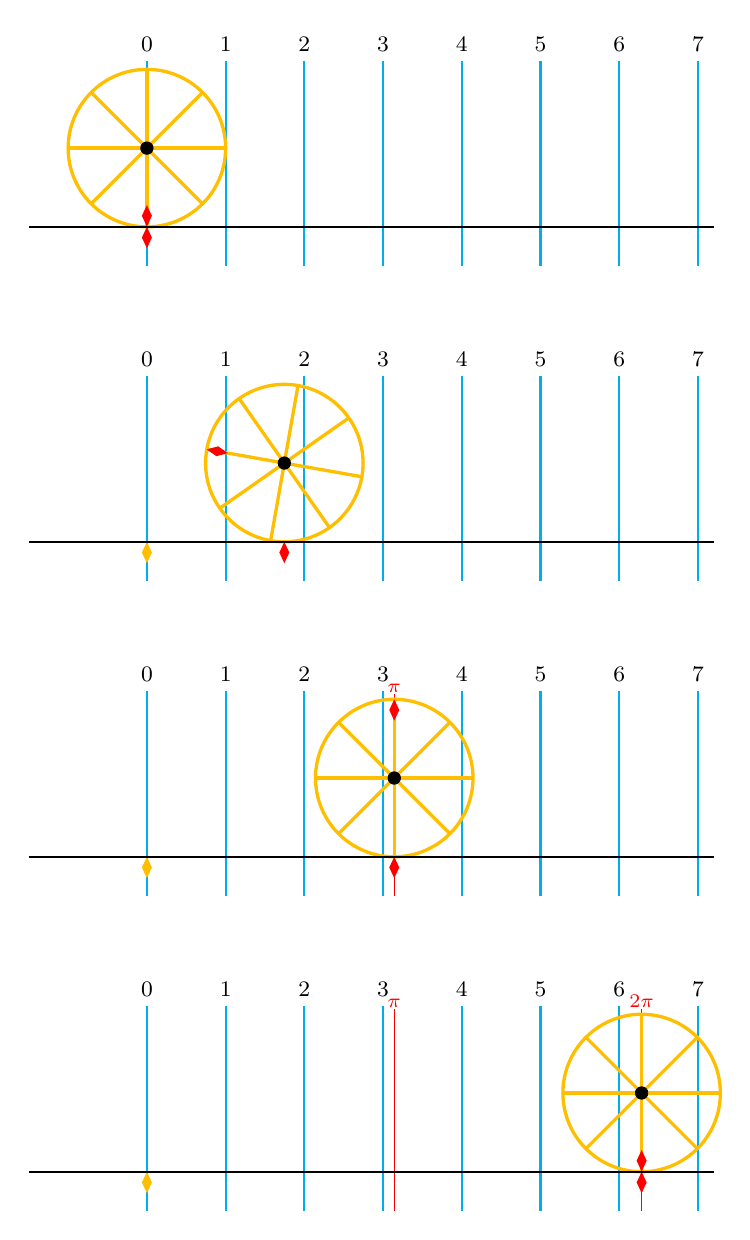
\begin{tikzpicture} 
\coordinate (O) at (0,0);
\coordinate (A) at (0,1);
\coordinate (B) at ($ (A) + cos(0)*(1,0) + sin(0)*(0,1) $);
\coordinate (C) at ($ (A) + cos(45)*(1,0) + sin(45)*(0,1) $);
\coordinate (D) at ($ (A) + cos(90)*(1,0) + sin(90)*(0,1) $);
\coordinate (E) at ($ (A) + cos(135)*(1,0) + sin(135)*(0,1) $);
\coordinate (F) at ($ (A) + cos(180)*(1,0) + sin(180)*(0,1) $);
\coordinate (G) at ($ (A) + cos(225)*(1,0) + sin(225)*(0,1) $);
\coordinate (H) at ($ (A) + cos(270)*(1,0) + sin(270)*(0,1) $);
\coordinate (I) at ($ (A) + cos(315)*(1,0) + sin(315)*(0,1) $);
\foreach \x in {0, 1, ..., 7}
 \draw[cyan, thick] ($ (O)+(\x,-.5) $)--++(0,2.6) node[anchor=south]{\footnotesize\color{black} \x};

\draw[orange!50!yellow, very thick] (A) circle (1cm);
\draw[orange!50!yellow, very thick] (B) -- (F);
\draw[orange!50!yellow, very thick] (C) -- (G);
\draw[orange!50!yellow, very thick] (D) -- (H);
\draw[orange!50!yellow, very thick] (E) -- (I);
\filldraw[black] (A) circle (2.2pt);
\coordinate (P) at ($ (H) + .15*cos(65)*(1,0)+.15*sin(70)*(0,1) $);
\coordinate (Q) at at ($ (P) + .15*cos(65)*(-1,0)+ .15* sin(65)*(0,1) $);
\coordinate (R) at at ($ (Q) + .15* cos(65)*(-1,0)+.15* sin(65)*(0,-1) $);
\draw[draw=none, fill=red] (H)--(P)--(Q)--(R)--cycle;

\coordinate (P) at ($ (H) + .15*cos(65)*(1,0)+.15*sin(65)*(0,-1) $);
\coordinate (Q) at at ($ (P) + .15*cos(65)*(-1,0)+ .15* sin(65)*(0,-1) $);
\coordinate (R) at at ($ (Q) + .15* cos(65)*(-1,0)+ .15* sin(65)*(0,1) $);
\draw[draw=none, fill=red] (H)--(P)--(Q)--(R)--cycle;
\draw[black, thick] (O)+(-1.5,0)--+(7.2,0);

%second fig
\coordinate (O) at (0,-4);
\coordinate (A) at ($ 100*pi/180*(1,0)+(0,-3) $);
\coordinate (B) at ($ (A) + cos(-100)*(1,0) + sin(-100)*(0,1) $);
\coordinate (C) at ($ (A) + cos(-55)*(1,0) + sin(-55)*(0,1) $);
\coordinate (D) at ($ (A) + cos(-10)*(1,0) + sin(-10)*(0,1) $);
\coordinate (E) at ($ (A) + cos(35)*(1,0) + sin(35)*(0,1) $);
\coordinate (F) at ($ (A) + cos(80)*(1,0) + sin(80)*(0,1) $);
\coordinate (G) at ($ (A) + cos(125)*(1,0) + sin(125)*(0,1) $);
\coordinate (H) at ($ (A) + cos(170)*(1,0) + sin(170)*(0,1) $);
\coordinate (I) at ($ (A) + cos(215)*(1,0) + sin(215)*(0,1) $);
\foreach \x in {0, 1, ..., 7}
 \draw[cyan, thick] ($ (O)+(\x,-.5) $)--++(0,2.6) node[anchor=south]{\footnotesize\color{black} \x};

\draw[orange!50!yellow, very thick] (A) circle (1cm);
\draw[orange!50!yellow, very thick] (B) -- (F);
\draw[orange!50!yellow, very thick] (C) -- (G);
\draw[orange!50!yellow, very thick] (D) -- (H);
\draw[orange!50!yellow, very thick] (E) -- (I);
\filldraw[black] (A) circle (2.2pt);
\coordinate (T) at ($ (A) + (0,-1) $);
\coordinate (P) at ($ (H) + .15*cos(-35)*(1,0)+.15* sin(-35)*(0,1) $);
\coordinate (Q) at at ($ (P) + .15*cos(15)*(1,0)+ .15* sin(15)*(0,1) $);
\coordinate (R) at at ($ (Q) + .15* cos(-35)*(-1,0)+.15* sin(-35)*(0,-1) $);
\draw[draw=none, fill=red] (H)--(P)--(Q)--(R)--cycle;
%red diamond on axis
\coordinate (P) at ($ (T) + .15*cos(65)*(1,0)+.15*sin(65)*(0,-1) $);
\coordinate (Q) at at ($ (P) + .15*cos(65)*(-1,0)+ .15* sin(65)*(0,-1) $);
\coordinate (R) at at ($ (Q) + .15* cos(65)*(-1,0)+ .15* sin(65)*(0,1) $);
\draw[draw=none, fill=red] (T)--(P)--(Q)--(R)--cycle;
%yellow diamond on axis
\coordinate (P) at ($ (O) + .15*cos(65)*(1,0)+.15*sin(65)*(0,-1) $);
\coordinate (Q) at at ($ (P) + .15*cos(65)*(-1,0)+ .15* sin(65)*(0,-1) $);
\coordinate (R) at at ($ (Q) + .15* cos(65)*(-1,0)+ .15* sin(65)*(0,1) $);
\draw[draw=none, fill=orange!50!yellow] (O)--(P)--(Q)--(R)--cycle;

\draw[black, thick] (O)+(-1.5,0)--+(7.2,0);

%fourth fig
\coordinate (O) at (0,-12);
\coordinate (A) at ($ 2* pi*(1,0)+(0,-11) $);
\coordinate (B) at ($ (A) + cos(0)*(1,0) + sin(0)*(0,1) $);
\coordinate (C) at ($ (A) + cos(45)*(1,0) + sin(45)*(0,1) $);
\coordinate (D) at ($ (A) + cos(90)*(1,0) + sin(90)*(0,1) $);
\coordinate (E) at ($ (A) + cos(135)*(1,0) + sin(135)*(0,1) $);
\coordinate (F) at ($ (A) + cos(180)*(1,0) + sin(180)*(0,1) $);
\coordinate (G) at ($ (A) + cos(225)*(1,0) + sin(225)*(0,1) $);
\coordinate (H) at ($ (A) + cos(270)*(1,0) + sin(270)*(0,1) $);
\coordinate (I) at ($ (A) + cos(315)*(1,0) + sin(315)*(0,1) $);
\foreach \x in {0, 1, ..., 7}
 \draw[cyan, thick] ($ (O)+(\x,-.5) $)--++(0,2.6) node[anchor=south]{\footnotesize\color{black} \x};

\draw[red] ($ (O)+(2*pi,-.5) $)--++(0,2.57) node[anchor=south, yshift=-3]{\scriptsize $2\pi$};
\draw[red] ($ (O)+(pi,-.5) $)--++(0,2.57) node[anchor=south, yshift=-3]{\scriptsize $\pi$};

\draw[orange!50!yellow, very thick] (A) circle (1cm);
\draw[orange!50!yellow, very thick] (B) -- (F);
\draw[orange!50!yellow, very thick] (C) -- (G);
\draw[orange!50!yellow, very thick] (D) -- (H);
\draw[orange!50!yellow, very thick] (E) -- (I);
\filldraw[black] (A) circle (2.2pt);
\coordinate (T) at ($ (A) + (0,-1) $);
\coordinate (P) at ($ (H) + .15*cos(65)*(1,0)+.15*sin(70)*(0,1) $);
\coordinate (Q) at at ($ (P) + .15*cos(65)*(-1,0)+ .15* sin(65)*(0,1) $);
\coordinate (R) at at ($ (Q) + .15* cos(65)*(-1,0)+.15* sin(65)*(0,-1) $);
\draw[draw=none, fill=red] (H)--(P)--(Q)--(R)--cycle;

%red diamond on axis
\coordinate (P) at ($ (T) + .15*cos(65)*(1,0)+.15*sin(65)*(0,-1) $);
\coordinate (Q) at at ($ (P) + .15*cos(65)*(-1,0)+ .15* sin(65)*(0,-1) $);
\coordinate (R) at at ($ (Q) + .15* cos(65)*(-1,0)+ .15* sin(65)*(0,1) $);
\draw[draw=none, fill=red] (T)--(P)--(Q)--(R)--cycle;
%yellow diamond on axis
\coordinate (P) at ($ (O) + .15*cos(65)*(1,0)+.15*sin(65)*(0,-1) $);
\coordinate (Q) at at ($ (P) + .15*cos(65)*(-1,0)+ .15* sin(65)*(0,-1) $);
\coordinate (R) at at ($ (Q) + .15* cos(65)*(-1,0)+ .15* sin(65)*(0,1) $);
\draw[draw=none, fill=orange!50!yellow] (O)--(P)--(Q)--(R)--cycle;

\draw[black, thick] (O)+(-1.5,0)--+(7.2,0);

%third fig
\coordinate (O) at (0,-8);
\coordinate (A) at ($ pi*(1,0)+(0,-7) $);
\coordinate (B) at ($ (A) + cos(-180)*(1,0) + sin(-180)*(0,1) $);
\coordinate (C) at ($ (A) + cos(-135)*(1,0) + sin(-135)*(0,1) $);
\coordinate (D) at ($ (A) + cos(-90)*(1,0) + sin(-90)*(0,1) $);
\coordinate (E) at ($ (A) + cos(-45)*(1,0) + sin(-45)*(0,1) $);
\coordinate (F) at ($ (A) + cos(0)*(1,0) + sin(0)*(0,1) $);
\coordinate (G) at ($ (A) + cos(45)*(1,0) + sin(45)*(0,1) $);
\coordinate (H) at ($ (A) + cos(90)*(1,0) + sin(90)*(0,1) $);
\coordinate (I) at ($ (A) + cos(135)*(1,0) + sin(135)*(0,1) $);
\foreach \x in {0, 1, ..., 7}
 \draw[cyan, thick] ($ (O)+(\x,-.5) $)--++(0,2.6) node[anchor=south]{\footnotesize\color{black} \x};

\draw[red] ($ (O)+(pi,-.5) $)--++(0,2.57) node[anchor=south, yshift=-3]{\scriptsize $\pi$};

\draw[orange!50!yellow, very thick] (A) circle (1cm);
\draw[orange!50!yellow, very thick] (B) -- (F);
\draw[orange!50!yellow, very thick] (C) -- (G);
\draw[orange!50!yellow, very thick] (D) -- (H);
\draw[orange!50!yellow, very thick] (E) -- (I);
\filldraw[black] (A) circle (2.2pt);
\coordinate (T) at ($ (A) + (0,-1) $);
\coordinate (P) at ($ (H) + .15*cos(65)*(1,0)+.15* sin(65)*(0,-1) $);
\coordinate (Q) at at ($ (P) + .15*cos(65)*(-1,0)+ .15* sin(65)*(0,-1) $);
\coordinate (R) at at ($ (Q) + .15* cos(65)*(-1,0)+ .15* sin(65)*(0,1) $);
\draw[draw=none, fill=red] (H)--(P)--(Q)--(R)--cycle;
%red diamond on axis
\coordinate (P) at ($ (T) + .15*cos(65)*(1,0)+.15*sin(65)*(0,-1) $);
\coordinate (Q) at at ($ (P) + .15*cos(65)*(-1,0)+ .15* sin(65)*(0,-1) $);
\coordinate (R) at at ($ (Q) + .15* cos(65)*(-1,0)+ .15* sin(65)*(0,1) $);
\draw[draw=none, fill=red] (T)--(P)--(Q)--(R)--cycle;
%yellow diamond on axis
\coordinate (P) at ($ (O) + .15*cos(65)*(1,0)+.15*sin(65)*(0,-1) $);
\coordinate (Q) at at ($ (P) + .15*cos(65)*(-1,0)+ .15* sin(65)*(0,-1) $);
\coordinate (R) at at ($ (Q) + .15* cos(65)*(-1,0)+ .15* sin(65)*(0,1) $);
\draw[draw=none, fill=orange!50!yellow] (O)--(P)--(Q)--(R)--cycle;

\draw[black, thick] (O)+(-1.5,0)--+(7.2,0);

\end{tikzpicture}
\newline
\subsection{6.1 Arclengths and Radians}

fig-6-1-intro
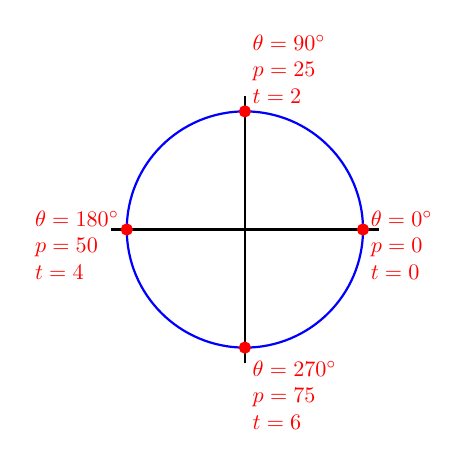
\begin{tikzpicture}

\coordinate (O) at (0,0);
\draw[blue,thick] (O) circle (1.5cm);
\coordinate (A) at (0:1.5);
\coordinate (B) at (90:1.5);
\coordinate (C) at (180:1.5);
\coordinate (D) at (270:1.5);

\draw[black,thick] (-1.7,0)--(1.7,0);
\draw[black,thick] (0,-1.7)--(0,1.7);

\filldraw[red] (A) circle (2.pt) node[anchor=west, align=left, yshift=-.2cm,scale=.8] {$\theta=0\degree$ \\ $p=0$ \\ $t=0$};
\filldraw[red] (B) circle (2.pt) node[anchor=south west, align=left,scale=.8] {$\theta=90\degree$ \\ $p=25$ \\ $t=2$};
\filldraw[red] (C) circle (2.pt) node[anchor=east, align=left, yshift=-.2cm,scale=.8] {$\theta=180\degree$ \\ $p=50$ \\ $t=4$};
\filldraw[red] (D) circle (2.pt) node[anchor=north west, align=left, yshift=-2, scale=.8] {$\theta=270\degree$ \\ $p=75$ \\ $t=6$};

\end{tikzpicture}
\newline

fig-6-1-arca
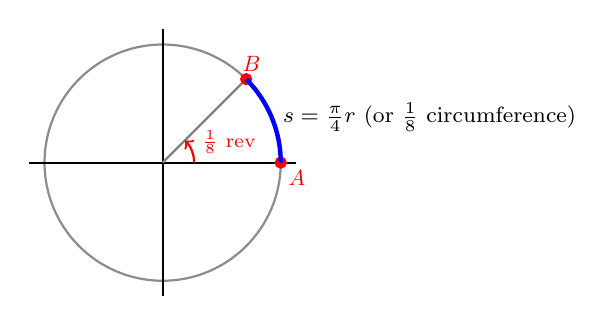
\begin{tikzpicture}

\coordinate (O) at (0,0);
\draw[gray!90!white,thick] (O) circle (1.5cm);
\coordinate (A) at (0:1.5);
\coordinate (B) at (45:1.5);

\draw[black,thick] (-1.7,0)--(1.7,0);
\draw[black,thick] (0,-1.7)--(0,1.7);
\draw[gray, thick] (O)--(B);

\filldraw[red] (A) circle (2.pt) node[anchor=north west, yshift=0,scale=.8] {$A$};
\filldraw[red] (B) circle (2.pt) node[anchor=south, xshift=2,scale=.8] {$B$};

\draw[red,thick,->](0.4,0) arc(0:45:.4) node[right, midway, yshift=3]{\scriptsize $\frac{1}{8}$ rev};
\draw[blue, ultra thick](1.5,0) arc(0:45:1.5) node[right, midway, color=black]{\footnotesize$s=\frac{\pi}{4}r$ (or $\frac{1}{8}$ circumference)};

\end{tikzpicture}
\newline

fig-6-1-arcb
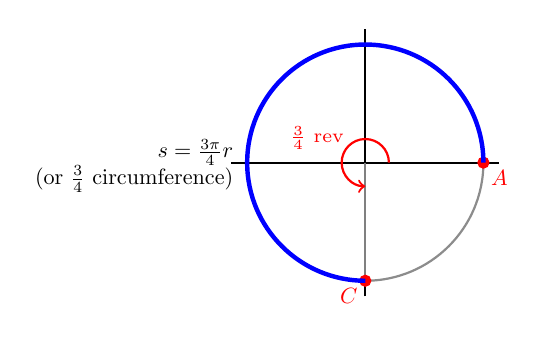
\begin{tikzpicture}

\coordinate (O) at (0,0);
\draw[gray!90!white,thick] (O) circle (1.5cm);
\coordinate (A) at (0:1.5);
\coordinate (C) at (270:1.5);

\draw[black,thick] (-1.7,0)--(1.7,0);
\draw[black,thick] (0,-1.7)--(0,1.7);
\draw[gray, thick] (O)--(C);

\filldraw[red] (A) circle (2.pt) node[anchor=north west, yshift=0,scale=.8] {$A$};
\filldraw[red] (C) circle (2.pt) node[anchor=north east, scale=.8] {$C$};

\draw[red,thick,->](0.3,0) arc(0:270:.3) node[above left, midway, xshift=2, yshift=-5]{\scriptsize $\frac{3}{4}$ rev};
\draw[blue, ultra thick](1.5,0) arc(0:270:1.5) node[left, midway, xshift=-.5cm, yshift=-1.1cm, align=right, scale=.8, text=black]{$s=\frac{3\pi}{4}r$ \\ (or $\frac{3}{4}$ circumference)};

\end{tikzpicture}
\newline


fig-6-1-arcc
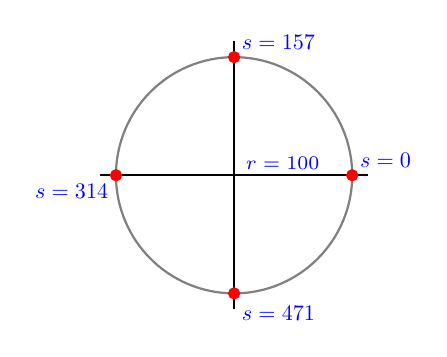
\begin{tikzpicture}

\coordinate (O) at (0,0);
\draw[gray,thick] (O) circle (1.5cm);
\coordinate (A) at (0:1.5);
\coordinate (B) at (90:1.5);
\coordinate (C) at (180:1.5);
\coordinate (D) at (270:1.5);

\draw[black,thick] (-1.7,0)--(1.7,0);
\draw[black,thick] (0,-1.7)--(0,1.7);

\filldraw[red] (A) circle (2.pt) node[anchor=south west, yshift=0,scale=.8, text=blue] {$s=0$};
\filldraw[red] (B) circle (2.pt) node[anchor=south west, align=left,scale=.8, text=blue] {$s=157$};
\filldraw[red] (C) circle (2.pt) node[anchor=east, align=left, yshift=-.2cm,scale=.8, text=blue] {$s=314$};
\filldraw[red] (D) circle (2.pt) node[anchor=north west, align=left, yshift=-2, scale=.8, text=blue] {$s=471$};
\node[text width=1.1cm,  text=blue] at (.7,.15){\scriptsize $r=100$};

\end{tikzpicture}
\newline

exam6-1-1
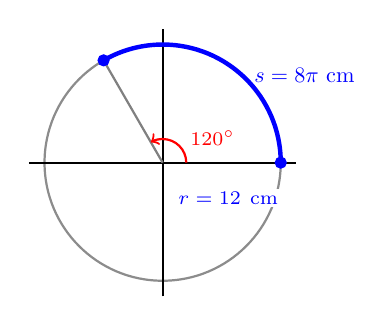
\begin{tikzpicture}

\coordinate (O) at (0,0);
\draw[gray!90!white,thick] (O) circle (1.5cm);
\coordinate (A) at (0:1.5);
\coordinate (B) at (120:1.5);

\draw[black,thick] (-1.7,0)--(1.7,0);
\draw[black,thick] (0,-1.7)--(0,1.7);
\draw[gray, thick] (O)--(B);

\filldraw[blue] (A) circle (2.pt);
\filldraw[blue] (B) circle (2.pt);

\draw[red,thick,->](0.3,0) arc(0:120:.3) node[above right, midway, xshift=2, yshift=-5]{\scriptsize $120\degree$};
\draw[blue, ultra thick](1.5,0) arc(0:120:1.5) node[above right, midway, xshift=.3cm, yshift=-.4cm, scale=.8]{$s=8\pi$ cm};
\node[text width=1.4cm, text=blue, fill=white, inner sep=1pt] at (.9,-.45){\scriptsize $r=12$ cm};

\end{tikzpicture}
\newline


fig-6-1-rad

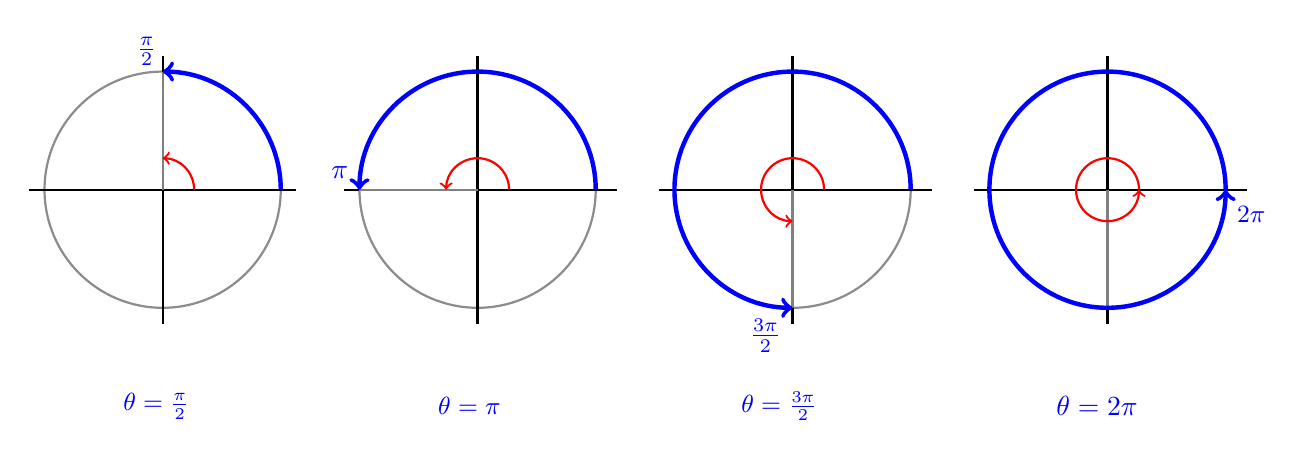
\begin{tikzpicture}

\coordinate (O) at (0,0);
\draw[gray!90!white,thick] (O) circle (1.5cm);
\coordinate (A) at (0:1.5);
\coordinate (B) at (90:1.5);

\draw[black,thick] (-1.7,0)--(1.7,0);
\draw[black,thick] (0,-1.7)--(0,1.7);
\draw[gray, thick] (O)--(B);

\draw[red,thick,->](0.4,0) arc(0:90:.4) ;
\draw[blue, ultra thick,->](1.5,0) arc(0:90:1.5) node[above left, xshift=2, yshift=-2]{$\frac{\pi}{2}$};
\node[text width=1cm, text=blue] at (0,-2.75){\small $\theta = \frac{\pi}{2}$};

%second circle
\coordinate (O) at (4,0);
\draw[gray!90!white,thick] (O) circle (1.5cm);
\coordinate (A) at ($ (O)+(1.5,0) $);
\coordinate (B) at ($ (O)+(-1.5,0) $);

\draw[black,thick] (O)++(-1.7,0)--++(3.47,0);
\draw[black,thick] (O)++(0,-1.7)--++(0,3.4);
\draw[gray, thick] (O)--(B);

\draw[red,thick,->](4.4,0) arc(0:180:.4) ;
\draw[blue, ultra thick,->](5.5,0) arc(0:180:1.5) node[above left, xshift=0, yshift=0]{$\small\pi$};
\node[text width=1cm, text=blue] at (4,-2.75){\small $\theta = \pi$};

%third circle
\coordinate (O) at (8,0);
\draw[gray!90!white,thick] (O) circle (1.5cm);
\coordinate (A) at ($ (O)+(1.5,0) $);
\coordinate (B) at ($ (O)+(0, -1.5) $);

\draw[black,thick] (O)++(-1.7,0)--++(3.47,0);
\draw[black,thick] (O)++(0,-1.7)--++(0,3.4);
\draw[gray, thick] (O)--(B);

\draw[red,thick,->](8.4,0) arc(0:270:.4) ;
\draw[blue, ultra thick,->](9.5,0) arc(0:270:1.5) node[below left, xshift=0, yshift=0]{$\frac{3\pi}{2}$};
\node[text width=1.3cm, text=blue] at (8,-2.75){\small $\theta = \frac{3\pi}{2}$};

%fourth circle
\coordinate (O) at (12,0);
\draw[gray!90!white,thick] (O) circle (1.5cm);
\coordinate (A) at ($ (O)+(1.5,0) $);
\coordinate (B) at ($ (O)+(0, -1.5) $);

\draw[black,thick] (O)++(-1.7,0)--++(3.47,0);
\draw[black,thick] (O)++(0,-1.7)--++(0,3.4);
\draw[gray, thick] (O)--(B);

\draw[red,thick,->](12.4,0) arc(0:360:.4) ;
\draw[blue, ultra thick,->](13.5,0) arc(0:360:1.5) node[below right, xshift=0, yshift=-2]{\small $2\pi$};
\node[text width=1.3cm, text=blue] at (12,-2.75){$\small \theta = 2\pi$};

\end{tikzpicture}
\newline


fig-6-1-decrad

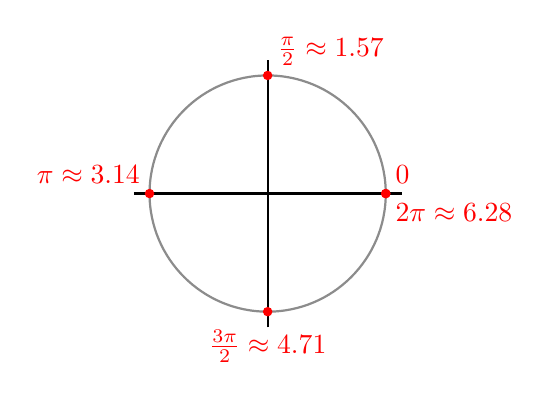
\begin{tikzpicture}

\coordinate (O) at (0,0);
\draw[gray!90!white,thick] (O) circle (1.5cm);
\coordinate (A) at (0:1.5);
\coordinate (B) at (90:1.5);
\coordinate (C) at (180:1.5);
\coordinate (D) at (270:1.5);

\draw[black,thick] (-1.7,0)--(1.7,0);
\draw[black,thick] (0,-1.7)--(0,1.7);
\draw[red, fill=red] (A) circle (1.5pt) node[anchor=south west] {0};
\draw[red, fill=red] (A) circle (1.5pt) node[anchor=north west] {$2\pi \approx 6.28$};
\draw[red, fill=red] (B) circle (1.5pt) node[anchor=south west] {$\frac{\pi}{2}\approx 1.57$};
\draw[red, fill=red] (C) circle (1.5pt) node[anchor=south east] {$\pi\approx 3.14$};
\draw[red, fill=red] (D) circle (1.5pt) node[anchor=north, yshift=-3] {$\frac{3\pi}{2}\approx 4.71$};

\end{tikzpicture}
\newline


fig-6-1-onerad

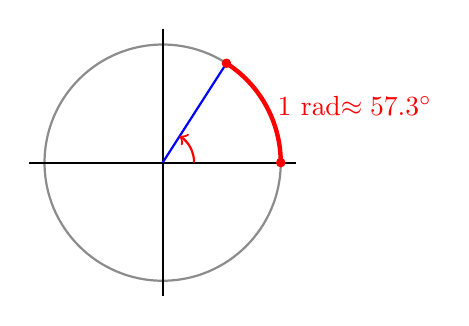
\begin{tikzpicture}

\coordinate (O) at (0,0);
\draw[gray!90!white,thick] (O) circle (1.5cm);
\coordinate (A) at (0:1.5);
\coordinate (B) at ($({deg(1)}:1.5) $);

\draw[black,thick] (-1.7,0)--(1.7,0);
\draw[black,thick] (0,-1.7)--(0,1.7);
\draw[blue,thick] (O)--(B);
\draw[red, fill=red] (A) circle (1.5pt);
\draw[red, thick, ->] (0.4,0) arc ((0:{deg(1)}:0.4) ;
\draw[red, fill=red] (B) circle (1.5pt);
\draw[red, ultra thick] (A) arc ((0:{deg(1)}:1.5) node[right, midway] {1 rad$\approx 57.3\degree$};

\end{tikzpicture}
\newline


fig6-1-radpro protractor

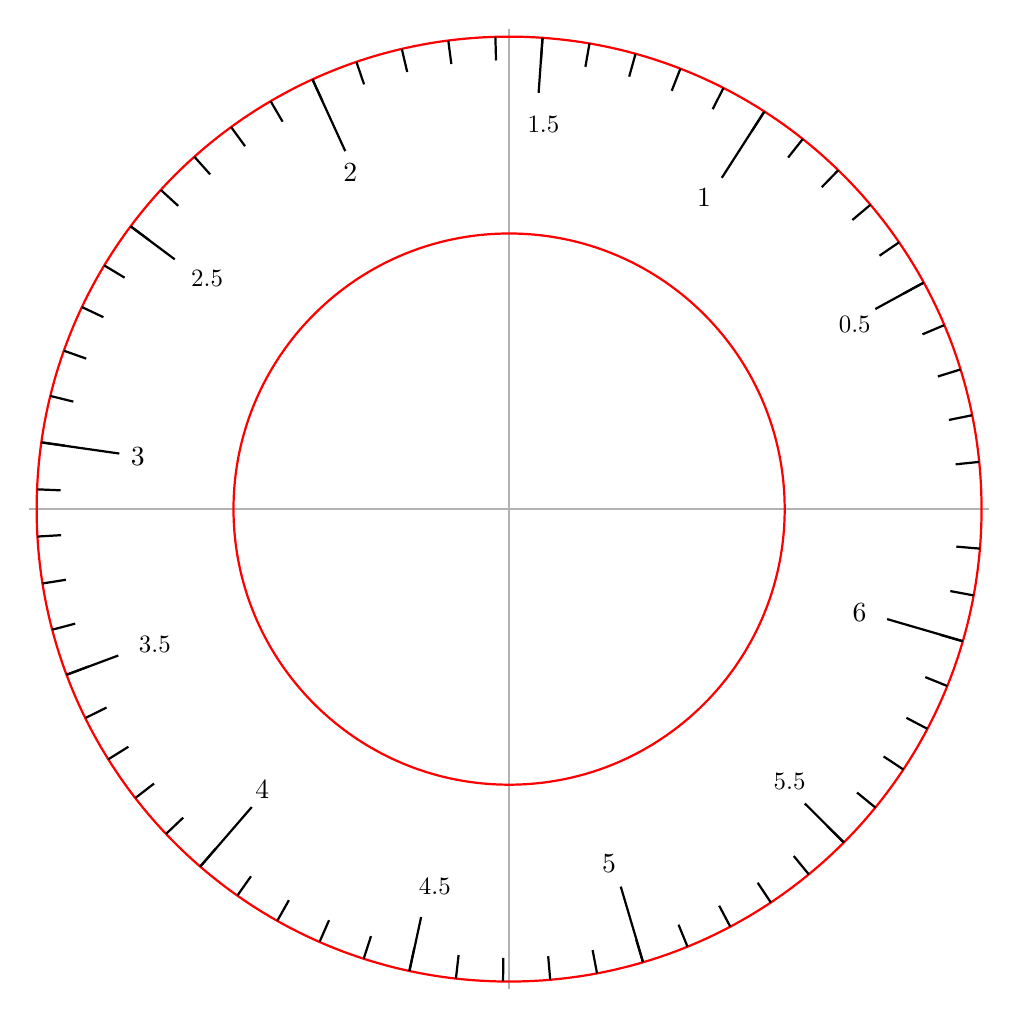
\begin{tikzpicture}

\coordinate (O) at (0,0);
\draw[gray!60!white, thick] (-6.1,0) --(6.1,0);
\draw[gray!60!white, thick] (0,-6.1) --(0, 6.1);

\draw[red, thick] (O) circle (3.5cm);
\draw[red, thick] (O) circle (6cm);

\foreach \i in {0.1, 0.2, ..., 6.2}
 \draw[black,thick] ({deg(\i)}:6)--({deg(\i)}:5.7);
\foreach \i in {1, 2, ..., 6}{
 \draw[black,thick] ({deg(\i)}:6)--({deg(\i)}:5);
 \node[text width=.3cm] at ({deg(\i}:4.7) {\i}; };
\foreach \i in {0.5,1.5, 2.5, ..., 5.5} {
 \draw[black,thick] ({deg(\i)}:6)--({deg(\i)}:5.3);
 \node[text width=.25cm, scale=.9] at ({deg(\i}:4.9) {\i}; };

\end{tikzpicture}
\newline


fig-6-1-arclength

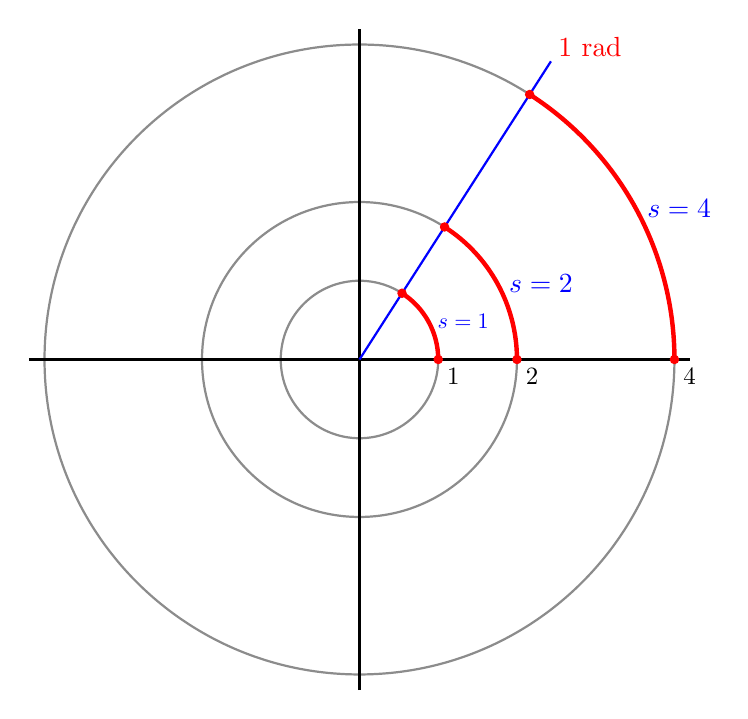
\begin{tikzpicture}

\coordinate (O) at (0,0);
\draw[gray!90!white,thick] (O) circle (1.cm);
\draw[gray!90!white,thick] (O) circle (2cm);
\draw[gray!90!white,thick] (O) circle (4cm);
\coordinate (A) at (0:1.);
\coordinate (B) at ($({deg(1)}:4.5) $);
\coordinate (Ab) at ($(0:2) $);
\coordinate (Ac) at ($(0:4) $);

\draw[black,thick] (-4.2,0)--(4.2,0);
\draw[black,thick] (0,-4.2)--(0,4.2);
\draw[blue,thick] (O)--(B) node[anchor=south west, xshift=-1, yshift=-2, text=red]{1 rad};
\draw[red, fill=red] (A) circle (1.5pt) node[anchor=north west, scale=.9, text=black]{1};
\draw[red, fill=red] ($({deg(1)}:1) $) circle (1.5pt);
\draw[red, ultra thick] (A) arc ((0:{deg(1)}:1) node[right, midway, scale=.8, text=blue] {$s=1$};

\draw[red, fill=red] (Ab) circle (1.5pt) node[anchor=north west, scale=.9, text=black]{2};
\draw[red, fill=red] ($({deg(1)}:2) $) circle (1.5pt);
\draw[red, ultra thick] (Ab) arc ((0:{deg(1)}:2) node[right, midway, text=blue] {$s=2$};

\draw[red, fill=red] (Ac) circle (1.5pt) node[anchor=north west, scale=.9, text=black]{4};
\draw[red, fill=red] ($({deg(1)}:4) $) circle (1.5pt);
\draw[red, ultra thick] (Ac) arc ((0:{deg(1)}:4) node[right, midway, text=blue] {$s=4$};

\end{tikzpicture}
\newline


exam6-1-5

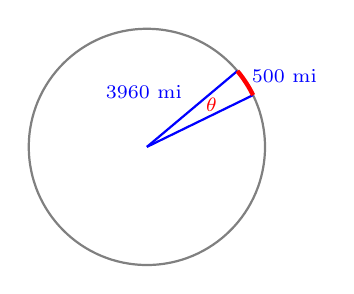
\begin{tikzpicture}

\coordinate (O) at (0,0);
\draw[gray, thick] (O) circle (1.5cm);

\coordinate (A) at (26:1.5);
\coordinate (B) at (40:1.5);

\draw[blue, thick] (A)--(O);
\draw[blue, thick] (O) --(B) node[above left, midway] {\scriptsize 3960 mi};

\draw[red, ultra thick] (A) arc(26:40:1.5) node[above right, midway, xshift=-2, yshift=-4, text=blue] {\scriptsize 500 mi};

\node[text width=.2 cm] at (32:1) {\color{red}\scriptsize$\theta$};

\end{tikzpicture}
\newline


exer6-1-3ans
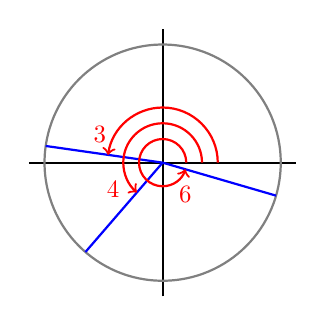
\begin{tikzpicture}

\coordinate (O) at (0,0);
\draw[black, thick] (-1.7,0)--(1.7,0);
\draw[black, thick] (0,-1.7)--(0,1.7);
\draw[gray, thick] (O) circle (1.5cm);

\coordinate (A) at ({deg(3)}:1.5);
\coordinate (B) at ({deg(4)}:1.5);
\coordinate (C) at ({deg(6)}:1.5);

\draw[blue, thick] (A)--(O);
\draw[red, thick, ->] (.7,0) arc (0:{deg(3)}:.7) node[above, xshift=-3, yshift=1, scale=.9]{3};
\draw[blue, thick] (B)--(O);
\draw[red, thick, ->] (.5,0) arc (0:{deg(4)}:.5) node[left, xshift=-3, yshift=1, scale=.9]{4};
\draw[blue, thick] (C)--(O);
\draw[red, thick, ->] (.3,0) arc (0:{deg(6)}:.3) node[below, yshift=-3, scale=.9]{6};

\end{tikzpicture}
\newline


hp6-1-1
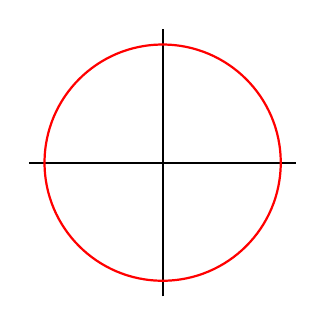
\begin{tikzpicture}

\coordinate (O) at (0,0);
\draw[black, thick] (-1.7,0)--(1.7,0);
\draw[black, thick] (0,-1.7)--(0,1.7);
\draw[red, thick] (O) circle (1.5cm);

\end{tikzpicture}
\newline



hp6-1-1ans
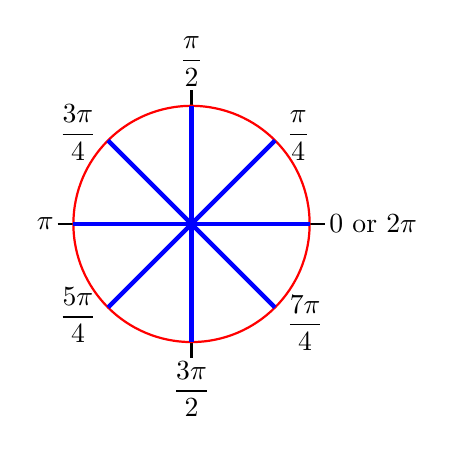
\begin{tikzpicture}

\coordinate (O) at (0,0);
\draw[black, thick] (-1.7,0)--(1.7,0);
\draw[black, thick] (0,-1.7)--(0,1.7);
\draw[red, thick] (O) circle (1.5cm);

\draw[blue,ultra thick] (O)--(0:1.5) node[anchor=west, xshift=3, text=black]{0 or $2\pi$};
\draw[blue,ultra thick] (O)--(45:1.5) node[anchor=south west, yshift=-.4cm, text=black]{$\displaystyle{\frac{\pi}{4}}$};
\draw[blue,ultra thick] (O)--(90:1.5) node[anchor=south , yshift=.1cm, text=black]{$\displaystyle{\frac{\pi}{2}}$};
\draw[blue,ultra thick] (O)--(135:1.5) node[anchor=south east, yshift=-.4cm, text=black]{$\displaystyle{\frac{3\pi}{4}}$};
\draw[blue,ultra thick] (O)--(180:1.5) node[anchor=east, xshift=-3, text=black]{$\pi$};
\draw[blue,ultra thick] (O)--(225:1.5) node[anchor=north east, yshift=.4cm, text=black]{$\displaystyle{\frac{5\pi}{4}}$};
\draw[blue,ultra thick] (O)--(270:1.5) node[anchor=north , yshift=-.1cm, text=black]{$\displaystyle{\frac{3\pi}{2}}$};
\draw[blue,ultra thick] (O)--(315:1.5) node[anchor=north west, yshift=.3cm, text=black]{$\displaystyle{\frac{7\pi}{4}}$};

\end{tikzpicture}
\newline


hp6-1-3
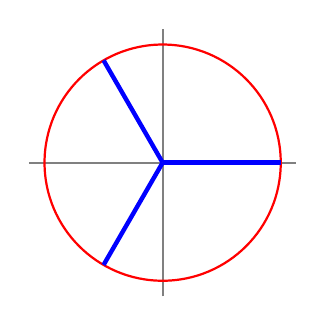
\begin{tikzpicture}

\coordinate (O) at (0,0);
\draw[gray, thick] (-1.7,0)--(1.7,0);
\draw[gray, thick] (0,-1.7)--(0,1.7);
\draw[red, thick] (O) circle (1.5cm);

\foreach \i in {0, 1, 2}
 \draw[blue,ultra thick] (O)--({\i*120}:1.5);

\end{tikzpicture}
\newline


hp6-1-4
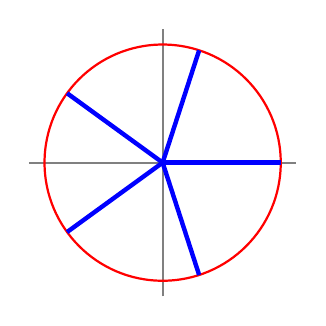
\begin{tikzpicture}

\coordinate (O) at (0,0);
\draw[gray, thick] (-1.7,0)--(1.7,0);
\draw[gray, thick] (0,-1.7)--(0,1.7);
\draw[red, thick] (O) circle (1.5cm);

\foreach \i in {0, 1, ..., 4}
 \draw[blue,ultra thick] (O)--({\i*72}:1.5);

\end{tikzpicture}
\newline


hp6-1-5
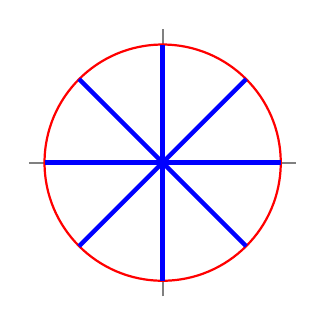
\begin{tikzpicture}

\coordinate (O) at (0,0);
\draw[gray, thick] (-1.7,0)--(1.7,0);
\draw[gray, thick] (0,-1.7)--(0,1.7);
\draw[red, thick] (O) circle (1.5cm);

\foreach \i in {0, 1, ..., 7}
 \draw[blue,ultra thick] (O)--({\i*45}:1.5);

\end{tikzpicture}
\newline


hp6-1-6
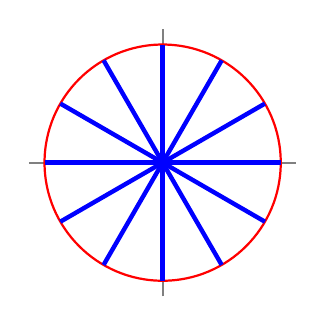
\begin{tikzpicture}

\coordinate (O) at (0,0);
\draw[gray, thick] (-1.7,0)--(1.7,0);
\draw[gray, thick] (0,-1.7)--(0,1.7);
\draw[red, thick] (O) circle (1.5cm);

\foreach \i in {0, 1, ..., 11}
 \draw[blue,ultra thick] (O)--({\i*30}:1.5);

\end{tikzpicture}
\newline


hp6-1-7
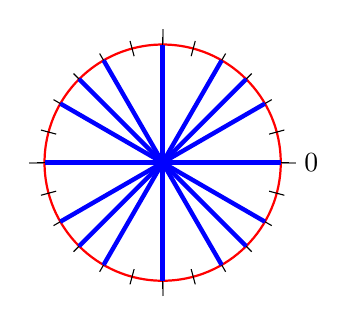
\begin{tikzpicture}

\coordinate (O) at (0,0);
\draw[gray, thick] (-1.7,0)--(1.7,0);
\draw[gray, thick] (0,-1.7)--(0,1.7);
\draw[red, thick] (O) circle (1.5cm);

\foreach \i in {0,15, ..., 345}
 \draw[black] (\i:1.4)--(\i:1.6);

\foreach \i in {0, 30,45,60,90,120,135,150,180, 210, 225, 240, 270, 300, 315, 330}
 \draw[blue,ultra thick] (O)--(\i:1.5);

\node[text width=.2cm] at (0:1.9) {0};

\end{tikzpicture}
\newline


hp6-1-7ans
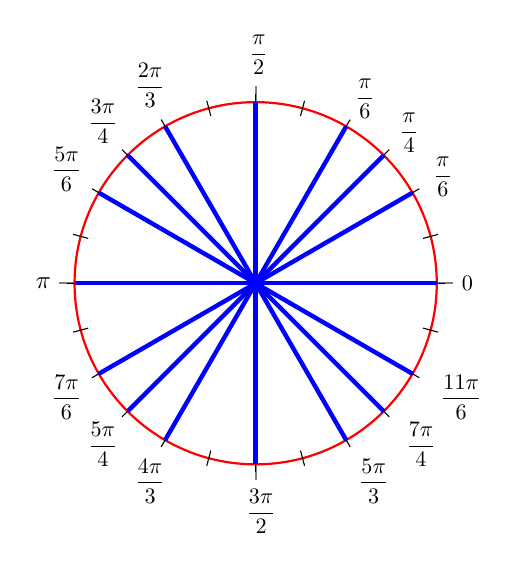
\begin{tikzpicture}

\coordinate (O) at (0,0);
\draw[gray, thick] (-2.5,0)--(2.5,0);
\draw[gray, thick] (0,-2.5)--(0,2.5);
\draw[red, thick] (O) circle (2.3cm);

\foreach \i in {0,15, ..., 345}
 \draw[black] (\i:2.2)--(\i:2.4);

\foreach \i in {0, 30,45,60,90,120,135,150,180, 210, 225, 240, 270, 300, 315, 330}
 \draw[blue,ultra thick] (O)--(\i:2.3);

\node[text width=.2cm, scale=.8] at (0:2.7) {0};
\node[text width=.2cm, scale=.8] at (30:2.7) {$\displaystyle{\frac{\pi}{6}}$};
\node[text width=.2cm, scale=.8] at (45:2.7) {$\displaystyle{\frac{\pi}{4}}$};
\node[text width=.2cm, scale=.8] at (60:2.7) {$\displaystyle{\frac{\pi}{6}}$};
\node[text width=.2cm, scale=.8] at (90:2.9) {$\displaystyle{\frac{\pi}{2}}$};
\node[text width=.2cm, scale=.8] at (120:2.9) {$\displaystyle{\frac{2\pi}{3}}$};
\node[text width=.2cm, scale=.8] at (135:2.9) {$\displaystyle{\frac{3\pi}{4}}$};
\node[text width=.2cm, scale=.8] at (150:2.9) {$\displaystyle{\frac{5\pi}{6}}$};
\node[text width=.2cm, scale=.9] at (180:2.7) {$\pi$};
\node[text width=.2cm, scale=.8] at (210:2.9) {$\displaystyle{\frac{7\pi}{6}}$};
\node[text width=.2cm, scale=.8] at (225:2.9) {$\displaystyle{\frac{5\pi}{4}}$};
\node[text width=.2cm, scale=.8] at (240:2.9) {$\displaystyle{\frac{4\pi}{3}}$};
\node[text width=.3cm, scale=.8] at (270:2.9) {$\displaystyle{\frac{3\pi}{2}}$};
\node[text width=.35cm, scale=.8] at (300:2.9) {$\displaystyle{\frac{5\pi}{3}}$};
\node[text width=.35cm, scale=.8] at (315:2.9) {$\displaystyle{\frac{7\pi}{4}}$};
\node[text width=.4cm, scale=.8] at (330:2.9) {$\displaystyle{\frac{11\pi}{6}}$};

\end{tikzpicture}
\newline


hp6-1-11

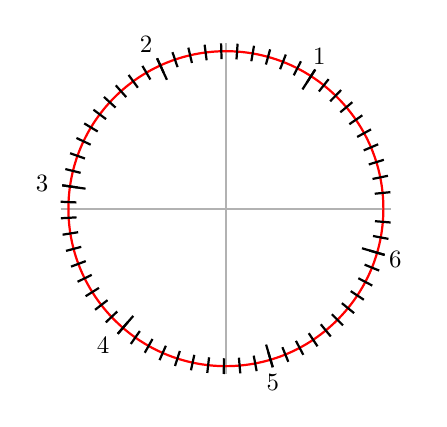
\begin{tikzpicture}

\coordinate (O) at (0,0);
\draw[gray!60!white, thick] (-2.1,0) --(2.1,0);
\draw[gray!60!white, thick] (0,-2.1) --(0, 2.1);

\draw[red, thick] (O) circle (2cm);

\foreach \i in {0.1, 0.2, ..., 6.2}
 \draw[black,thick] ({deg(\i)}:1.9)--({deg(\i)}:2.1);
\foreach \i in {1, 2, ..., 6}{
 \draw[black,thick] ({deg(\i)}:1.8)--({deg(\i)}:2.1);
 \node[text width=.3cm, scale=.9] at ({deg(\i}:2.3) {\i}; };

\end{tikzpicture}
\newline


hp6-1-11ans

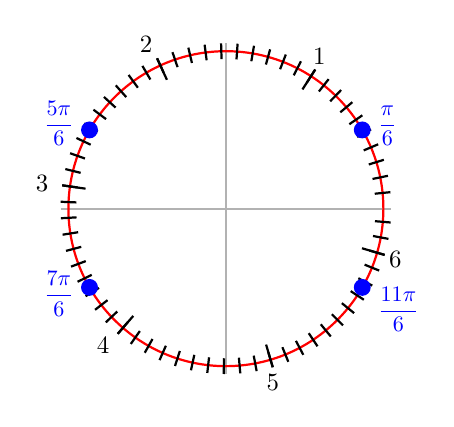
\begin{tikzpicture}

\coordinate (O) at (0,0);
\draw[gray!60!white, thick] (-2.1,0) --(2.1,0);
\draw[gray!60!white, thick] (0,-2.1) --(0, 2.1);

\draw[red, thick] (O) circle (2cm);

\foreach \i in {0.1, 0.2, ..., 6.2}
 \draw[black,thick] ({deg(\i)}:1.9)--({deg(\i)}:2.1);
\foreach \i in {1, 2, ..., 6}{
 \draw[black,thick] ({deg(\i)}:1.8)--({deg(\i)}:2.1);
 \node[text width=.3cm, scale=.9] at ({deg(\i}:2.3) {\i}; };

\filldraw[blue] (30:2) circle (.1cm) node[above right, xshift=.1cm, yshift=-.3cm, scale=.8]  {$\displaystyle{\frac{\pi}{6}}$};
\filldraw[blue] (150:2) circle (.1cm) node[above left, xshift=-.1cm, yshift=-.3cm, scale=.8]  {$\displaystyle{\frac{5\pi}{6}}$};
\filldraw[blue] (210:2) circle (.1cm) node[below left, xshift=-.1cm, yshift=.3cm, scale=.8]  {$\displaystyle{\frac{7\pi}{6}}$};
\filldraw[blue] (330:2) circle (.1cm) node[below right, xshift=.1cm, yshift=.1cm, scale=.8]  {$\displaystyle{\frac{11\pi}{6}}$};

\end{tikzpicture}
\newline


hp6-1-47 unit circle 
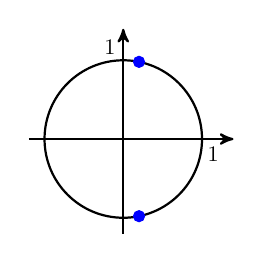
\begin{tikzpicture} 
\draw[black, thick,->, >=stealth'] (-1.2,0)-- (1.4,0);
\draw[black, thick, ->, >=stealth'] (0,-1.2) --(0,1.4);
\draw[black,thick] (0,0) circle (1cm);
\node[below right, scale=.8, xshift=-1] at (1,0) {1};
\node[above left, scale=.8, yshift=-1] at (0,1) {1};
\filldraw[blue] (0.2,0.98) circle (2pt);
\filldraw[blue] (0.2,-0.98) circle (2pt);

\end{tikzpicture}
\newline


hp6-1-49 unit circle 
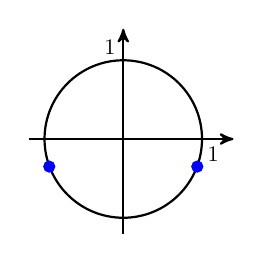
\begin{tikzpicture} 
\draw[black, thick,->, >=stealth'] (-1.2,0)-- (1.4,0);
\draw[black, thick, ->, >=stealth'] (0,-1.2) --(0,1.4);
\draw[black,thick] (0,0) circle (1cm);
\node[below right, scale=.8, xshift=-1] at (1,0) {1};
\node[above left, scale=.8, yshift=-1] at (0,1) {1};
\filldraw[blue] (0.94,-0.35) circle (2pt);
\filldraw[blue] (-0.94,-0.35) circle (2pt);

\end{tikzpicture}
\newline


hp6-1-51 unit circle 
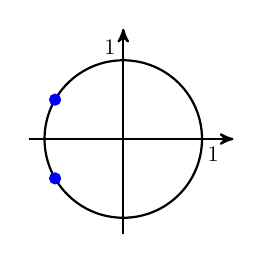
\begin{tikzpicture} 
\draw[black, thick,->, >=stealth'] (-1.2,0)-- (1.4,0);
\draw[black, thick, ->, >=stealth'] (0,-1.2) --(0,1.4);
\draw[black,thick] (0,0) circle (1cm);
\node[below right, scale=.8, xshift=-1] at (1,0) {1};
\node[above left, scale=.8, yshift=-1] at (0,1) {1};
\filldraw[blue] ({-sqrt(3)/2},1/2) circle (2pt);
\filldraw[blue] ({-sqrt(3)/2},-1/2) circle (2pt);

\end{tikzpicture}
\newline


hp6-1-53 grid
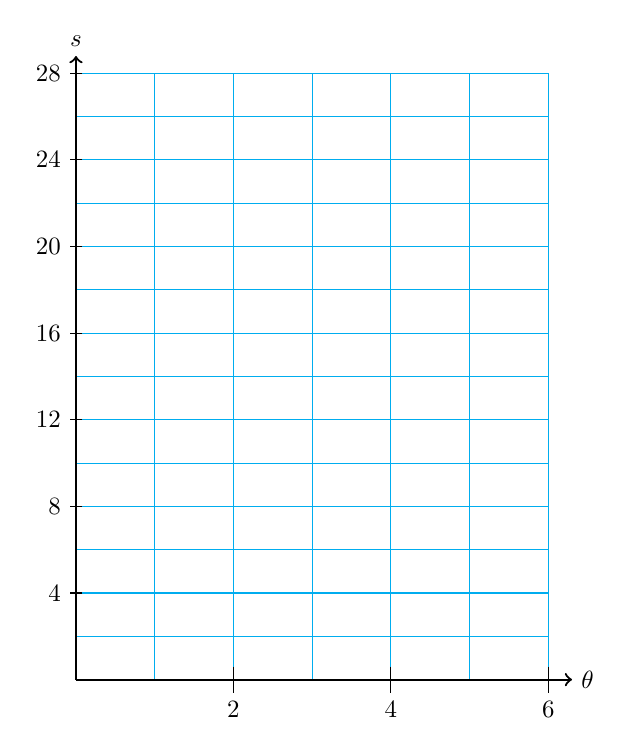
\begin{tikzpicture} [yscale=.55]

\draw[cyan] (0,0) grid (6,14);
\draw[black, thick,->] (0,0)-- (6.3,0) node[right, scale=.9]{$\theta$};
\draw[black, thick, ->] (0,0) --(0,14.4) node[above, scale=.9]{$s$};

\foreach \x in {2, 4, 6}
 \draw[black] (\x,.3) -- ++(0,-.6) node[below, scale=.9]{\x};

\foreach \y [evaluate=\y as \yi using int(2*\y)] in {2, 4, ..., 14} 
 \draw[black] (.08,\y)--++(-.16,0) node[left, scale=.9]{\yi};

\end{tikzpicture}
\newline


hp6-1-53ans

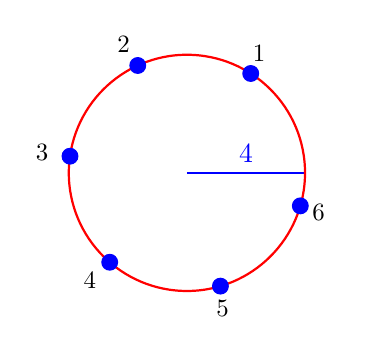
\begin{tikzpicture}

\coordinate (O) at (0,0);
\draw[blue, thick] (O) --(1.5,0) node[above, midway]{4};

\draw[red, thick] (O) circle (1.5cm);

\foreach \i in {1, 2, ..., 6}{
 \filldraw[blue] ({deg(\i}:1.5) circle (.1cm);
 \node[text width=.3cm, scale=.9] at ({deg(\i}:1.8) {\i}; };

\end{tikzpicture}
\newline


hp6-1-53ansc grid
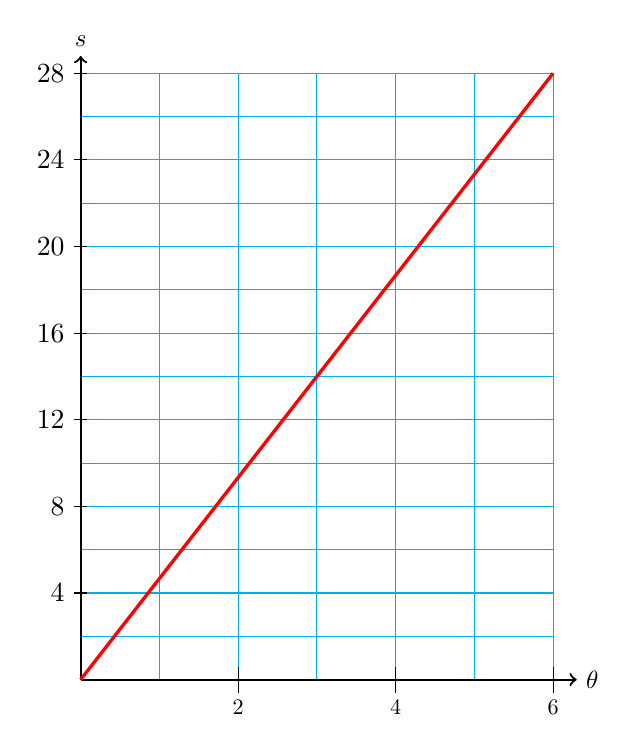
\begin{tikzpicture} [yscale=.55]

\draw[cyan] (0,0) grid (6,14);
\draw[black, thick,->] (0,0)-- (6.3,0) node[right, scale=.9]{$\theta$};
\draw[black, thick, ->] (0,0) --(0,14.4) node[above, scale=.9]{$s$};

\foreach \x in {2, 4, 6}
 \draw[black] (\x,.3) -- ++(0,-.6) node[below, scale=.8]{\x};

\foreach \y [evaluate=\y as \yi using int(2*\y)] in {2, 4, ..., 14} 
 \draw[black] (.08,\y)--++(-.16,0) node[left]{\yi};

\draw[red, very thick] (0,0) -- (6,14);

\end{tikzpicture}
\newline


hp6-1-54 grid
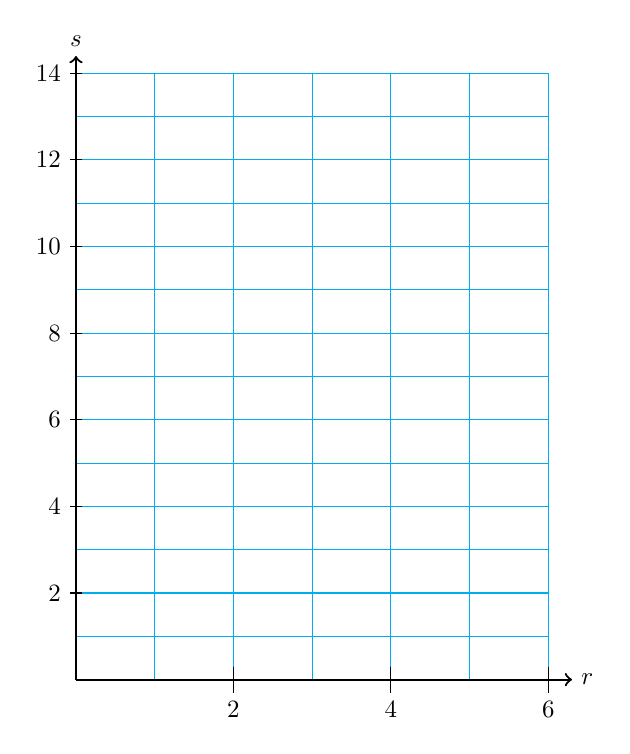
\begin{tikzpicture} [yscale=.55]

\draw[cyan] (0,0) grid (6,14);
\draw[black, thick,->] (0,0)-- (6.3,0) node[right, scale=.9]{$r$};
\draw[black, thick, ->] (0,0) --(0,14.4) node[above, scale=.9]{$s$};

\foreach \x in {2, 4, 6}
 \draw[black] (\x,.3) -- ++(0,-.6) node[below, scale=.9]{\x};

\foreach \y [evaluate=\y as \yi using int(\y)] in {2, 4, ..., 14} 
 \draw[black] (.08,\y)--++(-.16,0) node[left, scale=.9]{\yi};

\end{tikzpicture}
\newline


hp6-1-58a
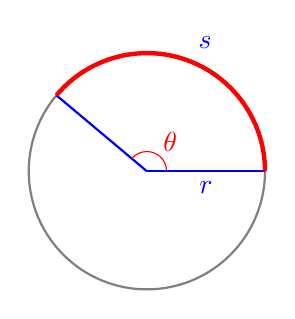
\begin{tikzpicture}

\coordinate (O) at (0,0);
\coordinate (A) at (1.5,0);
\coordinate (B) at (140:1.5);
\draw[gray, thick] (O) circle (1.5cm);
\draw[blue, thick] (B)--(O);
\draw[blue, thick] (O)--(A) node[below, midway] {$r$};
\draw[red, ultra thick] (A) arc (0:140:1.5) node[above right, midway, text=blue]{$s$};
\draw[red] (0.25,0) arc(0:140:0.25) node[above right, midway, yshift=-3] {$\theta$};

\end{tikzpicture}
\newline


hp6-1-58b
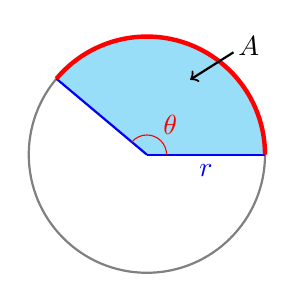
\begin{tikzpicture}

\coordinate (O) at (0,0);
\coordinate (A) at (1.5,0);
\coordinate (B) at (140:1.5);
\filldraw[cyan!40] (B)--(O)--(A) arc(0:140:1.5) ;
\draw[gray, thick] (O) circle (1.5cm);
\draw[blue, thick] (B)--(O);
\draw[blue, thick] (O)--(A) node[below, midway] {$r$};
\draw[red, ultra thick] (A) arc (0:140:1.5) ;
\draw[red] (0.25,0) arc(0:140:0.25) node[above right, midway, yshift=-3] {$\theta$};
\draw[black, thick, <-] (60:1.1)--(1.1,1.3) node[above right, xshift=-2, yshift=-5]{$A$};

\end{tikzpicture}
\newline


hp6-1-59
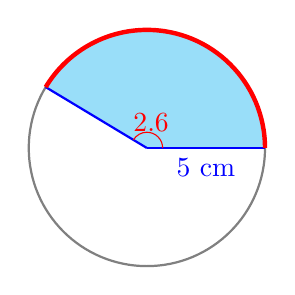
\begin{tikzpicture}

\coordinate (O) at (0,0);
\coordinate (A) at (1.5,0);
\coordinate (B) at ({deg(2.6)}:1.5);
\filldraw[cyan!40] (B)--(O)--(A) arc(0:{deg(2.6)}:1.5) ;
\draw[gray, thick] (O) circle (1.5cm);
\draw[blue, thick] (B)--(O);
\draw[blue, thick] (O)--(A) node[below, midway] {5 cm};
\draw[red, ultra thick] (A) arc (0:{deg(2.6)}:1.5) ;
\draw[red] (0.2,0) arc(0:{deg(2.6)}:0.2) node[above, midway, yshift=-3] {$2.6$};

\end{tikzpicture}
\newline


hp6-1-60
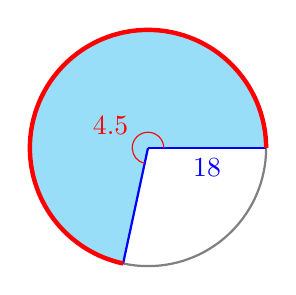
\begin{tikzpicture}

\coordinate (O) at (0,0);
\coordinate (A) at (1.5,0);
\coordinate (B) at ({deg(4.5)}:1.5);
\filldraw[cyan!40] (B)--(O)--(A) arc(0:{deg(4.5)}:1.5) ;
\draw[gray, thick] (O) circle (1.5cm);
\draw[blue, thick] (B)--(O);
\draw[blue, thick] (O)--(A) node[below, midway] {18};
\draw[red, ultra thick] (A) arc (0:{deg(4.5)}:1.5) ;
\draw[red] (0.2,0) arc(0:{deg(4.5)}:0.2) node[above left, midway, yshift=-3] {$4.5$};

\end{tikzpicture}
\newline


6-2-rads
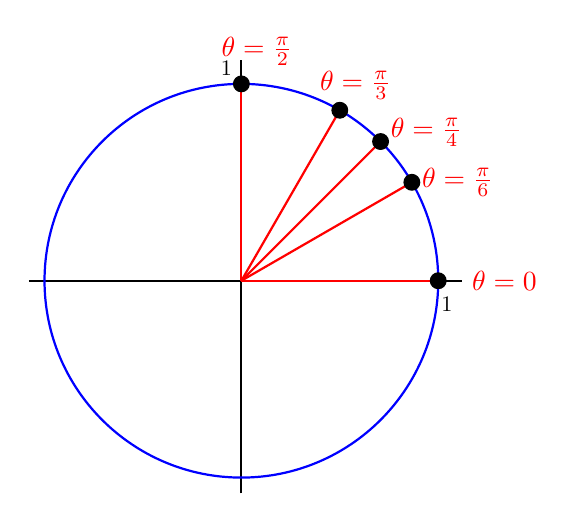
\begin{tikzpicture}

\coordinate (O) at (0,0);
\coordinate (A) at (0:2.5);
\coordinate (B) at (30:2.5);
\coordinate (C) at (45:2.5);
\coordinate (D) at (60:2.5);
\coordinate (E) at (90:2.5);

\draw[black, thick] (-2.7,0)--(2.8,0);
\draw[black, thick] (0,-2.7)--(0,2.8);
\draw[blue, thick] (O) circle (2.5);

\draw[red, thick] (O)--(A) node[right, xshift=.3cm]{$\theta = 0$};
\draw[red, thick] (O)--(B) node[right]{$\theta = \frac{\pi}{6}$};
\draw[red, thick] (O)--(C) node[above right, yshift=-.2cm]{$\theta = \frac{\pi}{4}$};
\draw[red, thick] (O)--(D) node[above, xshift=.2cm]{$\theta = \frac{\pi}{3}$};
\draw[red, thick] (O)--(E) node[above, xshift=.2cm, yshift=.1cm]{$\theta = \frac{\pi}{2}$};

\filldraw[black] (A) circle (.1cm);
\filldraw[black] (B) circle (.1cm);
\filldraw[black] (C) circle (.1cm);
\filldraw[black] (D) circle (.1cm);
\filldraw[black] (E) circle (.1cm);

\node[text width=.15cm, scale=.8] at (2.6,-.3) {1};
\node[text width=.15cm, scale=.8] at (-.2,2.7) {1};

\end{tikzpicture}
\newline

fig-6-2refang
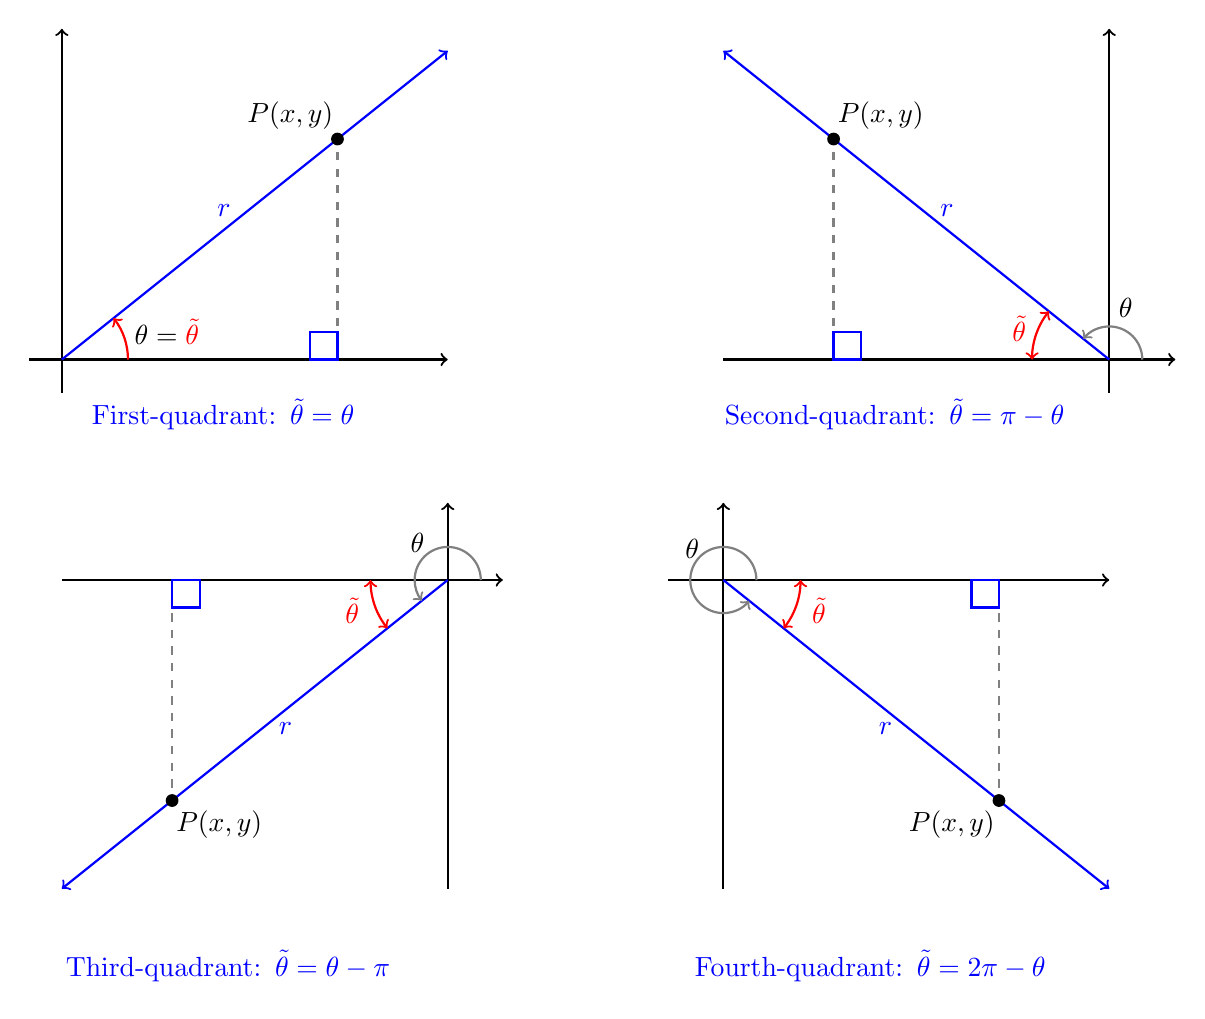
\begin{tikzpicture}[scale=1.4]

\coordinate (O) at (0,0);
\coordinate (x) at (2.5,0);
\coordinate (P) at (2.5,2);
\coordinate (A) at (3.5,0);
\coordinate (B) at (0,3);
\coordinate (C) at (3.5,2.8);

\draw[black,  thick, ->] (O)++(-.3,0) --(A);
\draw[black,  thick, ->] (O)++(0,-.3) -- (B) ;
\draw[blue,  thick, ->] (O) --  (C) node[left, midway, xshift=-5, yshift=-2]{$r$}  ;
\draw[red, thick, ->] (.6,0) arc (0:{atan(2/2.5)}:.6) node [right, midway,xshift=0,yshift=2] {$\color{black}\theta=\color{red}\tilde{\theta}$};

\draw[gray, thick, dashed] (x) -- (P);
\draw[blue, thick] (x) rectangle +(-.25,.25);

\filldraw (P) circle (1.5pt) node[anchor = south east, xshift=2]{$P(x,y)$}; 

\node[text width=4cm] at (1.7,-.5)     {\color{blue} First-quadrant: $\tilde{\theta}=\theta$};

%second quadrant


\coordinate (O) at (9.5,0);
\coordinate (x) at (7,0);
\coordinate (P) at (7,2);
\coordinate (A) at (6,0);
\coordinate (B) at (9.5,3);
\coordinate (C) at (6,2.8);

\draw[black,  thick, <-] (O)++(.6,0) --(A);
\draw[black,  thick, ->] (O)++(0,-.3) -- (B) ;
\draw[blue,  thick, ->] (O) --  (C) node[right, midway, xshift=5, yshift=-2]{$r$}  ;

\draw[red, thick, <->] (O)++(-.7,0) arc (180:{180-atan(2/2.5)}:.7) node [left, midway,xshift=0,yshift=2] {$\tilde{\theta}$};
\draw[gray, thick, ->] (O)++(.3,0) arc (0:{180-atan(2/2.5)}:.3) node [above, midway,xshift=2,yshift=0] {\color{black}$\theta$};

\draw[gray, thick, dashed] (x) -- (P);
\draw[blue, thick] (x) rectangle +(.25,.25);

\filldraw (P) circle (1.5pt) node[anchor = south west, xshift=-2]{$P(x,y)$}; 

\node[text width=5.cm] at (7.8,-.5)     {\color{blue} Second-quadrant: $\tilde{\theta}=\pi-\theta$};

%third quadrant

\coordinate (O) at (3.5,-2);
\coordinate (x) at (1,-2);
\coordinate (P) at (1,-4);
\coordinate (A) at (0,-2);
\coordinate (B) at (3.5,-4.8);
\coordinate (C) at (0,-4.8);

\draw[black,  thick, <-] (O)++(.5,0) --(A);
\draw[black,  thick, <-] (O)++(0,.7) -- (B) ;
\draw[blue,  thick, ->] (O) --  (C) node[right, midway, xshift=5, yshift=2]{$r$}  ;
\draw[red, thick, <->] (O)++(-.7,0) arc (180:{180+atan(2/2.5)}:.7) node [left, midway,xshift=-2,yshift=-2] {$\tilde{\theta}$};
\draw[gray, thick, ->] (O)++(.3,0) arc (0:{180+atan(2/2.5)}:.3) node [above, midway,xshift=-7,yshift=-5] {\color{black}$\theta$};

\draw[gray, thick, dashed] (x) -- (P);
\draw[blue, thick] (x) rectangle +(.25,-.25);

\filldraw (P) circle (1.5pt) node[anchor = north west, xshift=-2]{$P(x,y)$}; 

\node[text width=5.5cm] at (2.,-5.5)     {\color{blue} Third-quadrant: $\tilde{\theta}=\theta-\pi$};

%fourth quadrant

\coordinate (O) at (6,-2);
\coordinate (x) at (8.5,-2);
\coordinate (P) at (8.5,-4);
\coordinate (A) at (9.5,-2);
\coordinate (B) at (6,-4.8);
\coordinate (C) at (9.5,-4.8);

\draw[black,  thick, ->] (O)++(-.5,0) --(A);
\draw[black,  thick, <-] (O)++(0,.7) -- (B) ;
\draw[blue,  thick, ->] (O) --  (C) node[left, midway, xshift=-5, yshift=2]{$r$}  ;
\draw[red, thick, <->] (O)++(.7,0) arc (0:{-atan(2/2.5)}:.7) node [right, midway,xshift=2,yshift=-2] {$\tilde{\theta}$};
\draw[gray, thick, ->] (O)++(.3,0) arc (0:{360-atan(2/2.5)}:.3) node [above, midway,xshift=0,yshift=0] {\color{black}$\theta$};

\draw[gray, thick, dashed] (x) -- (P);
\draw[blue, thick] (x) rectangle +(-.25,-.25);

\filldraw (P) circle (1.5pt) node[anchor = north east, xshift=2]{$P(x,y)$}; 

\node[text width=5.2cm] at (7.6,-5.5)     {\color{blue} Fourth-quadrant: $\tilde{\theta}=2\pi -\theta$};

\end{tikzpicture}
\newline


act6-1
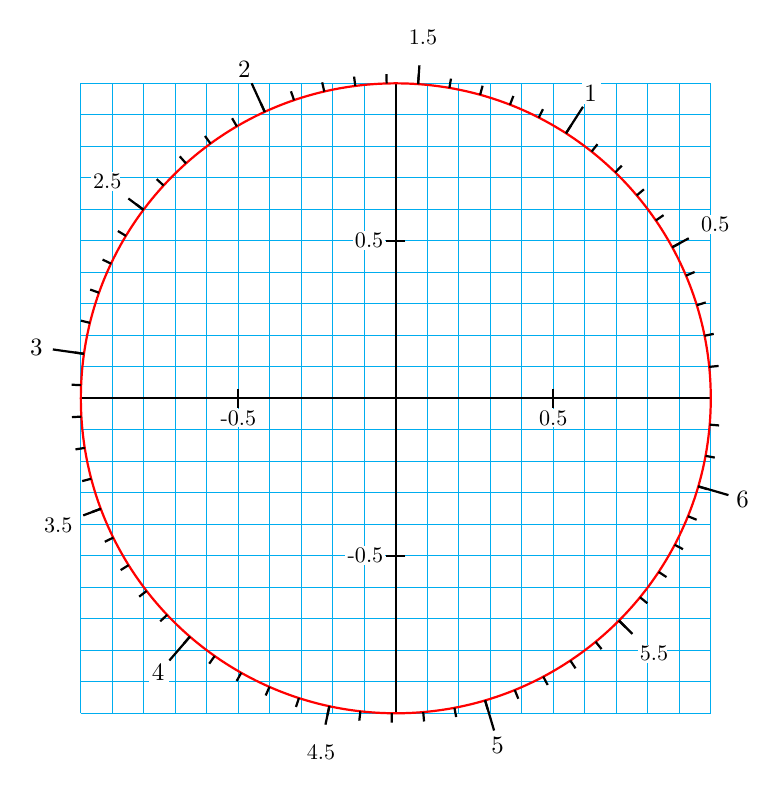
\begin{tikzpicture} [scale=4]

\draw[cyan] (-1.0001,-1.0001) grid[step = 0.1] (1,1);
\draw[black, thick] (-1,0)--(1,0);
\draw[black, thick] (0,-1)--(0,1);

\draw[red,thick] (0,0) circle (1cm);

\foreach \i in {0.1, 0.2, ..., 6.2} {
 \draw[black, thick] ({deg(\i)}:1) -- ({deg(\i)}:1.03);
};
\foreach \i in {0.5, 1.5, ..., 5.5} {
 \draw[black, thick] ({deg(\i)}:1) -- ({deg(\i)}:1.06);
 \node[text width=.4cm, fill=white, inner sep=1, scale=.8] at ({deg(\i)}:1.15) { \i};
};
\foreach \i in {1,2, ..., 6} {
 \draw[black, thick] ({deg(\i)}:1) -- ({deg(\i)}:1.1);
 \node[text width=.2cm, fill=white, inner sep=1, scale=.9] at ({deg(\i)}:1.15) { \i};
};
\foreach \i in {-0.5, 0.5} {
 \draw[black, thick] (0.03,\i) -- (-0.03,\i) node[left, fill=white, inner sep=1, scale=.8]{ \i};
 \draw[black, thick] (\i,0.03) -- (\i,-0.03) node[below, fill=white, inner sep=1, scale=.8]{\i};
};

\end{tikzpicture}
\newline


exam6-2-2a
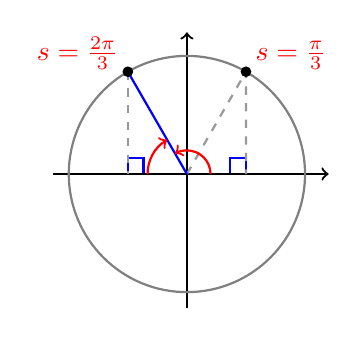
\begin{tikzpicture}

\coordinate (O) at (0,0);
\coordinate (A) at (60:1.5);
\coordinate (B) at (120:1.5);
\coordinate (C) at (0.75,0);
\coordinate (D) at (-0.75,0);

\draw[blue,thick] (C) rectangle ++(-.2,.2);
\draw[blue,thick] (D) rectangle ++(.2,.2);

\draw[black, thick, ->] (-1.7,0)--(1.8,0);
\draw[black, thick, ->] (0,-1.7)--(0,1.8);
\draw[gray, thick] (O) circle (1.5);

\draw[gray!80, thick, dashed] (O)--(A)--(C);
\draw[blue, thick] (O)--(B) ;
\draw[gray!80, thick, dashed] (B)--(D) ;
\draw[red, thick, ->] (0.3,0) arc(0:120:0.3);
\draw[red, thick, ->] (-0.5,0) arc(180:120:0.5);
\filldraw[black] (A) circle (.06cm) node[anchor=south west, yshift=-0.1cm, text=red] {$s=\frac{\pi}{3}$};
\filldraw[black] (B) circle (.06cm) node[anchor=south east, yshift=-0.1cm, text=red] {$s=\frac{2\pi}{3}$};

\end{tikzpicture}
\newline


exam6-2-2b
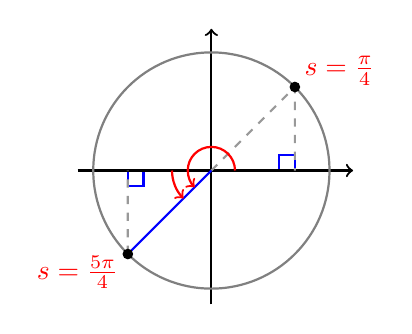
\begin{tikzpicture}

\coordinate (O) at (0,0);
\coordinate (A) at (45:1.5);
\coordinate (B) at (225:1.5);
\coordinate (C) at ($ sqrt(2)*(.75,0) $);
\coordinate (D) at ($ -sqrt(2)*(.75,0) $);

\draw[blue,thick] (C) rectangle ++(-.2,.2);
\draw[blue,thick] (D) rectangle ++(.2,-.2);

\draw[black, thick, ->] (-1.7,0)--(1.8,0);
\draw[black, thick, ->] (0,-1.7)--(0,1.8);
\draw[gray, thick] (O) circle (1.5);

\draw[gray!80, thick, dashed] (O)--(A)--(C);
\draw[blue, thick] (O)--(B) ;
\draw[gray!80, thick, dashed] (B)--(D) ;
\draw[red, thick, ->] (0.3,0) arc(0:225:0.3);
\draw[red, thick, ->] (-0.5,0) arc(180:225:0.5);
\filldraw[black] (A) circle (.06cm) node[anchor=south west, yshift=-0.1cm, text=red] {$s=\frac{\pi}{4}$};
\filldraw[black] (B) circle (.06cm) node[anchor=north east, yshift=0.1cm, text=red] {$s=\frac{5\pi}{4}$};

\end{tikzpicture}
\newline


fig-6-2-realnos
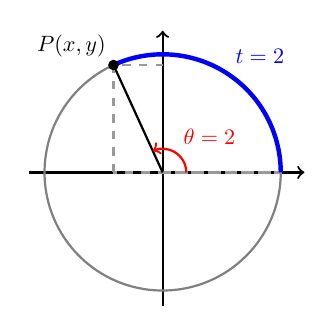
\begin{tikzpicture}

\coordinate (O) at (0,0);
\coordinate (A) at (0:1.5);
\coordinate (B) at ($({deg(2)}:1.5)$);
\coordinate (C) at ($ 1.5*cos(deg(2))*(1,0) $);
\coordinate (D) at ($ 1.5*sin(deg(2))*(0,1) $);

\draw[black, thick, ->] (-1.7,0)--(1.8,0);
\draw[black, thick, ->] (0,-1.7)--(0,1.8);
\draw[gray, thick] (O) circle (1.5);

\draw[gray!80, thick, dashed] (O)--(A)--(C);
\draw[black, thick] (O)--(B) ;
\draw[gray!80, thick, dashed] (C)--(B)--(D) ;
\draw[red, thick, ->] (0.3,0) arc(0:{deg(2)}:0.3)  node[above right, midway, scale=.8] {$\theta=2$};
\draw[blue, ultra thick] (1.5,0) arc(0:{deg(2)}:1.5)  node[above right, midway, scale=.8 ] {$t=2$};
\filldraw[black] (B) circle (.06cm) node[anchor=south east, scale=.8] { $P(x,y)$};

\end{tikzpicture}
\newline


fig-6-2-coords
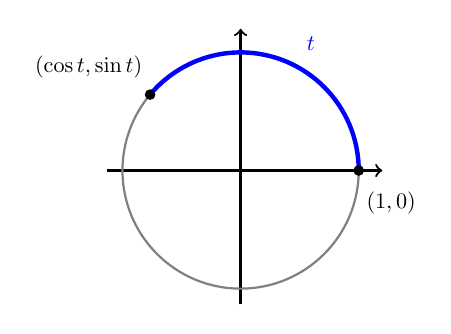
\begin{tikzpicture}

\coordinate (O) at (0,0);
\coordinate (A) at (0:1.5);
\coordinate (B) at (140:1.5);

\draw[black, thick, ->] (-1.7,0)--(1.8,0);
\draw[black, thick, ->] (0,-1.7)--(0,1.8);
\draw[gray, thick] (O) circle (1.5);

\draw[blue, ultra thick] (1.5,0) arc(0:140:1.5)  node[above right, midway, xshift=6, scale=.8 ] {$t$};
\filldraw[black] (A) circle (.06cm) node[anchor=north west, yshift=-5, scale=.8] { $(1,0)$};
\filldraw[black] (B) circle (.06cm) node[anchor=south east, yshift=3, scale=.8] { $(\cos t, \sin t)$};

\end{tikzpicture}
\newline


exam6-2-4a

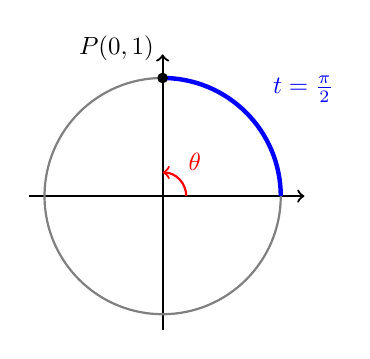
\begin{tikzpicture}

\coordinate (O) at (0,0);
\coordinate (A) at (0:1.5);
\coordinate (B) at (90:1.5);

\draw[black, thick, ->] (-1.7,0)--(1.8,0);
\draw[black, thick, ->] (0,-1.7)--(0,1.8);
\draw[gray, thick] (O) circle (1.5);

\draw[red, thick, ->] (0.3,0) arc(0:90:0.3)  node[above right, midway, scale=.9] {$\theta$};
\draw[blue, ultra thick] (1.5,0) arc(0:90:1.5)  node[above right, midway, xshift=6, scale=.9 ] {$t=\frac{\pi}{2}$};
\filldraw[black] (B) circle (.06cm) node[anchor=south east, yshift=3, scale=.9] { $P(0,1)$};

\end{tikzpicture}
\newline


exam6-2-4b
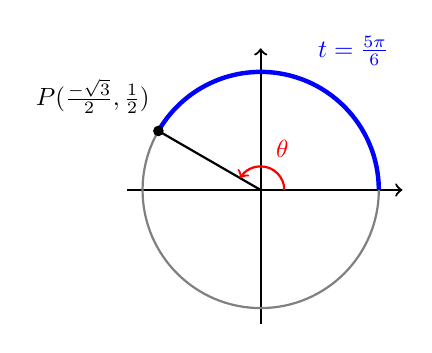
\begin{tikzpicture}

\coordinate (O) at (0,0);
\coordinate (A) at (0:1.5);
\coordinate (B) at (150:1.5);

\draw[black, thick, ->] (-1.7,0)--(1.8,0);
\draw[black, thick, ->] (0,-1.7)--(0,1.8);
\draw[black, thick] (O)--(B);
\draw[gray, thick] (O) circle (1.5);

\draw[red, thick, ->] (0.3,0) arc(0:150:0.3)  node[above right, midway, scale=.9] {$\theta$};
\draw[blue, ultra thick] (1.5,0) arc(0:150:1.5)  node[above right, midway, xshift=6, scale=.9 ] {$t=\frac{5\pi}{6}$};
\filldraw[black] (B) circle (.06cm) node[anchor=south east, yshift=3, scale=.9] { $P(\frac{-\sqrt{3}}{2}, \frac{1}{2})$};

\end{tikzpicture}
\newline


fig-6-2-tan

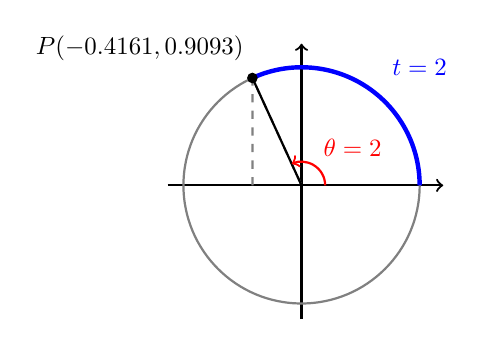
\begin{tikzpicture}

\coordinate (O) at (0,0);
\coordinate (A) at (0:1.5);
\coordinate (B) at ($ ({deg(2)}:1.5) $);
\coordinate (C) at ($ 1.5*cos(deg(2))*(1,0) $);
\coordinate (D) at ($ 1.5*sin(deg(2))*(0,0) $);

\draw[black, thick, ->] (-1.7,0)--(1.8,0);
\draw[black, thick, ->] (0,-1.7)--(0,1.8);
\draw[gray, thick, dashed] (C)--(B)--(D);
\draw[black, thick] (O)--(B);
\draw[gray, thick] (O) circle (1.5);

\draw[red, thick, ->] (0.3,0) arc(0:{deg(2)}:0.3)  node[above right, midway, scale=.9] {$\theta=2$};
\draw[blue, ultra thick] (1.5,0) arc(0:{deg(2)}:1.5)  node[above right, midway, xshift=6, scale=.9 ] {$t=2$};
\filldraw[black] (B) circle (.06cm) node[anchor=south east, yshift=3, scale=.9] { $P(-0.4161,0.9093)$};

\end{tikzpicture}
\newline


fig-6-2-circfun
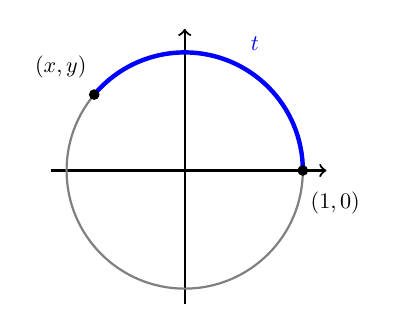
\begin{tikzpicture}

\coordinate (O) at (0,0);
\coordinate (A) at (0:1.5);
\coordinate (B) at (140:1.5);

\draw[black, thick, ->] (-1.7,0)--(1.8,0);
\draw[black, thick, ->] (0,-1.7)--(0,1.8);
\draw[gray, thick] (O) circle (1.5);

\draw[blue, ultra thick] (1.5,0) arc(0:140:1.5)  node[above right, midway, xshift=6, scale=.8 ] {$t$};
\filldraw[black] (A) circle (.06cm) node[anchor=north west, yshift=-5, scale=.8] { $(1,0)$};
\filldraw[black] (B) circle (.06cm) node[anchor=south east, yshift=3, scale=.8] { $(x,y)$};

\end{tikzpicture}
\newline


exam6-2-5
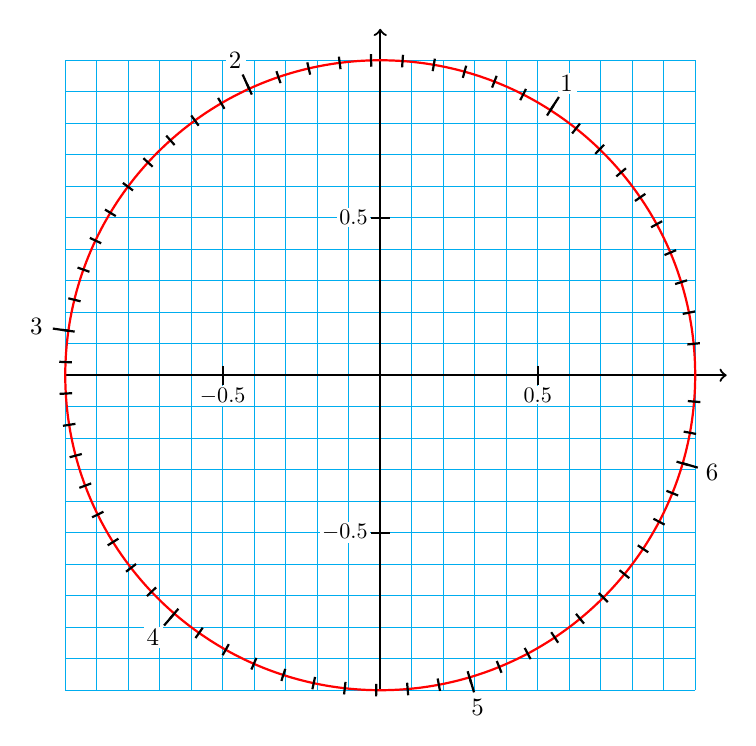
\begin{tikzpicture} [scale=4]

\draw[cyan] (-1.0001,-1.0001) grid[step = 0.1] (1,1);
\draw[black, thick, ->] (-1,0)--(1.1,0);
\draw[black, thick, ->] (0,-1)--(0,1.1);

\draw[red,thick] (0,0) circle (1cm);

\foreach \i in {0.1, 0.2, ..., 6.2} {
 \draw[black, thick] ({deg(\i)}:.98) -- ({deg(\i)}:1.02);
};
\foreach \i in {1,2, ..., 6} {
 \draw[black, thick] ({deg(\i)}:1) -- ({deg(\i)}:1.05);
 \node[text width=.2cm, fill=white, inner sep=1, scale=.9] at ({deg(\i)}:1.1) { $\i$};
};
\foreach \i in {-0.5, 0.5} {
 \draw[black, thick] (0.03,\i) -- (-0.03,\i) node[left, fill=white, inner sep=1, scale=.8]{ $\i$};
 \draw[black, thick] (\i,0.03) -- (\i,-0.03) node[below, fill=white, inner sep=1, scale=.8]{$\i$};
};

\end{tikzpicture}
\newline


hp6-2-1
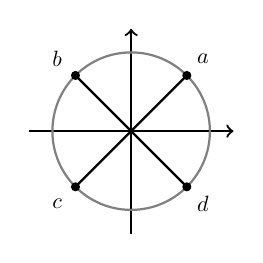
\begin{tikzpicture} 
\draw[black, thick, ->] (-1.3,0)--(1.3,0);
\draw[black, thick, ->] (0,-1.3)--(0,1.3);

\draw[gray,thick] (0,0) circle (1cm);

\foreach \i in {45, 135, 225, 315} {
 \draw[black, thick] (\i:1) -- (0,0);
 \filldraw[black] (\i:1) circle (0.05cm);
};

\node [text width=.2cm, scale=0.8] at (45:1.3) {$a$};
\node [text width=.2cm, scale=0.8] at (135:1.3) {$b$};
\node [text width=.2cm, scale=0.8] at (225:1.3) {$c$};
\node [text width=.2cm, scale=0.8] at (315:1.3) {$d$};
\end{tikzpicture}
\newline


hp6-2-2
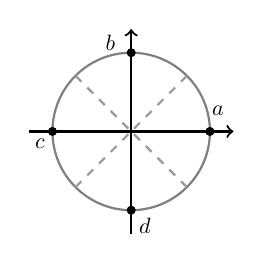
\begin{tikzpicture} 
\draw[black, thick, ->] (-1.3,0)--(1.3,0);
\draw[black, thick, ->] (0,-1.3)--(0,1.3);

\draw[gray,thick] (0,0) circle (1cm);

\foreach \i in {45, 135, 225, 315} {
 \draw[gray!80, thick, dashed] (\i:1) -- (0,0);
};

\filldraw[black] (1,0) circle (0.05cm) node [anchor=south west, xshift=-2, yshift=3, scale=0.8]  {$a$};
\filldraw[black] (0,1) circle (0.05cm) node [anchor=south east, xshift=-3, yshift=-2, scale=0.8]  {$b$};
\filldraw[black] (-1,0) circle (0.05cm) node [anchor=north east, scale=0.8]  {$c$};
\filldraw[black] (0,-1) circle (0.05cm) node [anchor=north west, scale=0.8]  {$d$};
\end{tikzpicture}
\newline


hp6-2-3
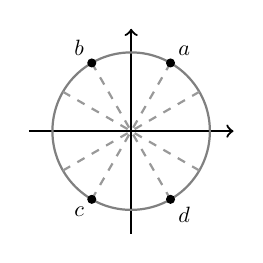
\begin{tikzpicture} 
\draw[black, thick, ->] (-1.3,0)--(1.3,0);
\draw[black, thick, ->] (0,-1.3)--(0,1.3);

\draw[gray,thick] (0,0) circle (1cm);

\foreach \i in {30, 60, 120, 150, 210, 240, 300, 330} {
 \draw[gray!80, thick, dashed] (\i:1) -- (0,0);
};

\filldraw[black] (60:1) circle (0.05cm) node [anchor=south west, scale=0.8]  {$a$};
\filldraw[black] (120:1) circle (0.05cm) node [anchor=south east, scale=0.8]  {$b$};
\filldraw[black] (240:1) circle (0.05cm) node [anchor=north east, scale=0.8]  {$c$};
\filldraw[black] (300:1) circle (0.05cm) node [anchor=north west, scale=0.8]  {$d$};
\end{tikzpicture}
\newline


hp6-2-4
\begin{tikzpicture} 
\draw[black, thick, ->] (-1.3,0)--(1.3,0);
\draw[black, thick, ->] (0,-1.3)--(0,1.3);

\draw[gray,thick] (0,0) circle (1cm);

\foreach \i in {30, 60, 120, 150, 210, 240, 300, 330} {
 \draw[gray!80, thick, dashed] (\i:1) -- (0,0);
};

\filldraw[black] (30:1) circle (0.05cm) node [anchor=south west, scale=0.8]  {$a$};
\filldraw[black] (150:1) circle (0.05cm) node [anchor=south east, scale=0.8]  {$b$};
\filldraw[black] (210:1) circle (0.05cm) node [anchor=north east, scale=0.8]  {$c$};
\filldraw[black] (330:1) circle (0.05cm) node [anchor=north west, scale=0.8]  {$d$};
\end{tikzpicture}
\newline


hp6-2-45ansa 
\begin{tikzpicture} [scale=1.5] 
\coordinate (O) at (0,0);
\draw[black, thick, ->] (-1.3,0)--(1.3,0);
\draw[black, thick, ->] (0,-1.3)--(0,1.3);

\draw[gray,thick] (O) circle (1cm);

\draw[black,thick] (O) -- (150:1);
\draw[black,thick] (O) -- (210:1);
\draw[black,thick] (O) -- (330:1);

\draw[red, thick, ->] (.2,0) arc(0:330:.2);
\draw[red, thick, ->] (.35,0) arc(0:210:.35);
\draw[red, thick, ->] (.5,0) arc(0:150:.5);

\node[text width = .15cm, anchor=north west, scale=.8] at (1,0) {$1$};
\node[text width = .15cm, anchor=south east, xshift=-1, scale=.8] at (0,1) {$1$};

\end{tikzpicture}
\newline


hp6-2-45ansb 
\begin{tikzpicture} [scale=1.5] 
\coordinate (O) at (0,0);
\draw[black, thick, ->] (-1.3,0)--(1.3,0);
\draw[black, thick, ->] (0,-1.3)--(0,1.3);

\draw[gray,thick] (O) circle (1cm);

\draw[black,thick] (O) -- (135:1);
\draw[black,thick] (O) -- (225:1);
\draw[black,thick] (O) -- (315:1);

\draw[red, thick, ->] (.2,0) arc(0:315:.2);
\draw[red, thick, ->] (.35,0) arc(0:225:.35);
\draw[red, thick, ->] (.5,0) arc(0:135:.5);

\node[text width = .15cm, anchor=north west, scale=.8] at (1,0) {$1$};
\node[text width = .15cm, anchor=south east, xshift=-1, scale=.8] at (0,1) {$1$};

\end{tikzpicture}
\newline


hp6-2-45ansc 
\begin{tikzpicture} [scale=1.5] 
\coordinate (O) at (0,0);
\draw[black, thick, ->] (-1.3,0)--(1.3,0);
\draw[black, thick, ->] (0,-1.3)--(0,1.3);

\draw[gray,thick] (O) circle (1cm);

\draw[black,thick] (O) -- (120:1);
\draw[black,thick] (O) -- (240:1);
\draw[black,thick] (O) -- (330:1);

\draw[red, thick, ->] (.2,0) arc(0:330:.2);
\draw[red, thick, ->] (.35,0) arc(0:240:.35);
\draw[red, thick, ->] (.5,0) arc(0:120:.5);

\node[text width = .15cm, anchor=north west, xshift=2, yshift=-3, scale=.8] at (1,0) {$1$};
\node[text width = .15cm, anchor=south east, xshift=-3, yshift=2, scale=.8] at (0,1) {$1$};

\end{tikzpicture}
\newline


hp6-2-67ans
\begin{tikzpicture} [scale=1.5] 
\coordinate (O) at (0,0);
\draw[black, thick, ->] (-1.3,0)--(1.3,0);
\draw[black, thick, ->] (0,-1.3)--(0,1.3);

\draw[gray,thick] (O) circle (1cm);
\draw[blue,thick] (-1.2,-1.2) --(1.05,1.05) node[above right, xshift=-1, yshift=-2, scale=.9]{$y=x$};

\filldraw[black] (45:1) circle (.03cm) node[anchor=west, xshift=.1cm] {$(\frac{1}{\sqrt{2}},\frac{1}{\sqrt{2}})$};
\filldraw[black] (225:1) circle (.03cm) node[anchor=north, xshift=.15cm, yshift=-.35cm] {$(\frac{-1}{\sqrt{2}},\frac{-1}{\sqrt{2}})$};

\end{tikzpicture}
\newline


hp6-2-69
\begin{tikzpicture} [scale=0.35] 
\draw[cyan] (-2,-2) grid (10,10);
\draw[black, thick, ->] (-2,0)--(10.8,0) node[right, scale=.9]{$x$};
\draw[black, thick, ->] (0,-2)--(0,10.8) node[above, scale=.9]{$y$};

\foreach \i in {-2,5,10} {
 \draw[black,thick] (\i,0.2)--++(0,-.4) node[below, scale=.8, fill=white, inner sep=2]{$\i$};
 \draw[black,thick] (.2, \i)--++(-.4,0) node[left, scale=.8, fill=white, inner sep=2]{$\i$};
}

\end{tikzpicture}
\newline


hp6-2-69ans
\begin{tikzpicture} [scale=0.35] 
\draw[cyan] (-2,-2) grid (10,10);
\draw[black, thick, ->] (-2,0)--(10.8,0) node[right, scale=.9]{$x$};
\draw[black, thick, ->] (0,-2)--(0,10.8) node[above, scale=.9]{$y$};

\foreach \i in {-2,5,10} {
 \draw[black,thick] (\i,0.2)--++(0,-.4) node[below, scale=.8, fill=white, inner sep=2]{$\i$};
 \draw[black,thick] (.2, \i)--++(-.4,0) node[left, scale=.8, fill=white, inner sep=2]{$\i$};
}
\coordinate (A) at (8,3);
\draw[red, thick] (-2,-.75)--(10,3.75);
\filldraw[black] (A) circle (.2cm);

\end{tikzpicture}
\newline


hp6-2-75
\begin{tikzpicture} [scale=1.2] 
\coordinate (O) at (0,0);
\coordinate (P) at (30:1);
\coordinate (Q) at ($ cos(30)*(1,0) $);
\coordinate (R) at (30:3);
\coordinate (S) at ($ 3*cos(30)*(1,0) $);
\draw[gray, thick] (O) circle (1cm);
\draw[gray!90, thick] (Q) rectangle ++(-.15,.15);
\draw[gray!90, thick] (S) rectangle ++(-.15,.15);
\draw[gray, thick] (P)--(Q);
\draw[gray, thick] (R)--(S);

\draw[black, thick] (-1.1,0)-- (S) ;
\draw[black, thick] (0,-1.1)--(0,1.2) ;

\draw[red, ultra thick] (1,0) arc(0:30:1) node[right, midway, text=black, scale=.8]{$t$};
\draw[blue,thick](O)--(R);
\filldraw[black] (P) circle (.03cm) node[above, scale=.8]{$P$};
\node[text width=.2cm, above, scale=.8] at (30:.5) {$1$};

\end{tikzpicture}
\newline


hp6-2-76
\begin{tikzpicture} [scale=1.2] 
\coordinate (O) at (0,0);
\coordinate (P) at (50:1);
\coordinate (Q) at ($ cos(50)*(1,0) $);
\coordinate (R) at ($ tan(50) *(0,1)+(1,0) $);
\coordinate (S) at (1,0);
\draw[gray, thick] (O) circle (1cm);
\draw[gray!90, thick] (Q) rectangle ++(-.15,.15);
\draw[gray!90, thick] (S) rectangle ++(.15,.15);
\draw[gray, thick] (P)--(Q);
\draw[gray, thick] (R)--(S);

\draw[black, thick] (-1.1,0)-- (1.3,0) ;
\draw[black, thick] (0,-1.1)--(0,1.5) ;

\draw[red, ultra thick] (1,0) arc(0:50:1) node[below left, midway, text=black, scale=.8]{$t$};
\draw[blue,thick](O)--(50:2.3);
\filldraw[black] (P) circle (.04cm);
\node[text width=.2cm, above, scale=.8] at (50:.5) {$1$};
\filldraw[black] (R) circle (.04cm) node[above left, scale=.8]{$T$};
\filldraw[black] (S) circle (.04cm) node[below right, scale=.8]{$S$};

\end{tikzpicture}
\newline


hp6-2-77
\begin{tikzpicture}  
\coordinate (O) at (0,0);
\coordinate (P) at (35:1);
\coordinate (Q) at ($ cos(35)*(1,0) $);
\coordinate (R) at (35:1.5);
\coordinate (S) at ($ 1.5*cos(35)*(1,0) $);
\draw[gray, thick] (O) circle (1cm);
\draw[gray, thick] (O) circle (1.5cm);
\draw[gray!90, thick] (Q) rectangle ++(-.15,.15);
\draw[gray!90, thick] (S) rectangle ++(.15,.15);
\draw[gray, thick] (P)--(Q);
\draw[gray, thick] (R)--(S);

\draw[black, thick, ->] (-1.7,0)-- (2.9,0) ;
\draw[black, thick, ->] (0,-1.6)--(0,1.9) ;

\draw[red, thick] (.3,0) arc(0:35:.3) node[right, midway, scale=.75]{$\theta$};
\draw[blue,thick](O)--(R);
\node[text width=.2cm, above, scale=.8] at (35:.5) {$1$};
\filldraw[black] (R) circle (.04cm) node[above right, scale=.8]{$P$};
\node[text width=2.1cm, scale=.8] at (2.1,-1.2) {$x^2+y^2=r^2$};

\end{tikzpicture}
\newline



\end{document}
